%---[ TEMPLATE: BOOK | monograph | mini-treatise ]
%---|original-author:JWL|date:24SEPT2025|email:jwl@nuchwezi.com
%---|TITLE: TEA TAZ – Transforming Executable Alphabet A: to Z: COMMAND SPACE SPECIFICATION
%---|EDITOR:Prof. Joseph Willrich Lutalo, Oxford
%---[MANUSCRIPT-VERSION:24SEPT2025]
%----------------------------------------------------------------|
%\documentclass[a4paper, 18pt]{article} % A4 paper, readable font size
\documentclass[a4paper, 18pt]{book} % A4 paper, readable font size
%\documentclass[a4paper, 18pt]{book} % A4 paper, readable font size
\usepackage{geometry} % Adjust margins
\geometry{top=0.8in, bottom=0.8in, left=0.8in, right=0.6in} 

\usepackage[utf8]{inputenc}


% packages we'll need...

% for about author styling
\usepackage{setspace}

% allow table of contents to also list subsections
\setcounter{tocdepth}{2}

% for better appendices
\usepackage[title,titletoc]{appendix}

% for controlling page numbers
\usepackage{fancyhdr}
\pagestyle{fancy}
\fancyhf{}
\fancyhead[R]{\thepage}

% throw in page-top header
\fancyhead[L]{TEA TAZ – Transforming Executable Alphabet A: to Z: COMMAND SPACE SPECIFICATION}

% for graphics
\usepackage{graphicx}
\usepackage{caption}
\usepackage{float}

%for multi-figure figures?
\usepackage{subcaption}


% for text-wrapping in verbatim environments
\usepackage{fvextra}
\RecustomVerbatimEnvironment{verbatim}{Verbatim}{breaklines, breakanywhere}

% for drawing text boxes

% for proper treatment of urls
\usepackage{hyperref}

% for tables
\usepackage{tabularx}

% for line-breaks in table cells
\usepackage{makecell}

% for diagonalsplit in table headers cell
\usepackage{diagbox}

% make table cells center vertically where we could have used p{1cm} -- we use m{1cm}
%\usepackage{array}
% alternatively, just use custom column type --- M{1cm}
%\newcolumntype{M}[1]{>{\centering\arraybackslash}m{#1}}


% for long tables
\usepackage{longtable}
% for custom table col widths
%\usepackage{array}
%\newcolumntype{L}{>{\centering\arraybackslash}m{2cm}}
%\newcolumntype{M}{>{\centering\arraybackslash}m{5cm}}

% for json listings...
%\usepackage{listings}
%\usepackage{minted}
%\usemintedstyle{xcode}% no parser errors in listings?
%\usemintedstyle{bw} % grayscale color in listings, but shows parser errors!

% for highlighting text
\usepackage{xcolor, soul}
% then define colors we shall use:
\definecolor{myteal}{RGB}{0, 128, 128}
\definecolor{lightgray}{HTML}{CCCCCC}
\definecolor{myorange}{HTML}{FFD7B3}

% for table with alternating row bg colors 
\usepackage[table]{xcolor}
\definecolor{lightgray}{gray}{0.9}  % or use HTML/RGB if preferred


%\definecolor{highcolor}{rgb}{0,255,255} % our default hl color for background, friendly on black text foreground
\definecolor{highcolor}{rgb}{0,255,255} %a accent background color, must be friendly on black text foreground
\sethlcolor{highcolor}

%for regular expression and TEA code presentation in console-like text-boxes
\usepackage{tcolorbox}
\tcbuselibrary{listings,skins,breakable}
\usepackage{listings}

% style for general terminal-like listings
\tcbset{
  myterminalstyle/.style={
    colback=black,       % background color
    coltext=white,       % text color
    fontupper=\ttfamily, % typewriter font
    boxrule=0pt,         % no border
    arc=0pt,             % square corners
    outer arc=0pt,
    left=2mm, right=2mm, top=1mm, bottom=1mm,
    enhanced,
    sharp corners,
  }
}

% define listings config for TEA language
\lstdefinelanguage{TEA}{
  morecomment=[l]{\#},
  sensitive=true,
  alsoletter={:*!},
  %morekeywords=[1]{i:, u!:, g:, l:, f:, x:, j:, q!:},
  morekeywords=[1]{%
a:, a.:, a*:, a!:, a.*:, a.!:, a*!:, b:, b.:, b*:, b!:, b.*:, b.!:, b*!:, c:, c.:, c*:, c!:, c.*:, c.!:, c*!:, d:, d.:, d*:, d!:, d.*:, d.!:, d*!:, e:, e.:, e*:, e!:, e.*:, e.!:, e*!:, f:, f.:, f*:, f!:, f.*:, f.!:, f*!:, g:, g.:, g*:, g!:, g.*:, g.!:, g*!:, h:, h.:, h*:, h!:, h.*:, h.!:, h*!:, i:, i.:, i*:, i!:, i.*:, i.!:, i*!:, j:, j.:, j*:, j!:, j.*:, j.!:, j*!:, k:, k.:, k*:, k!:, k.*:, k.!:, k*!:, l:, l.:, l*:, l!:, l.*:, l.!:, l*!:, m:, m.:, m*:, m!:, m.*:, m.!:, m*!:, n:, n.:, n*:, n!:, n.*:, n.!:, n*!:, o:, o.:, o*:, o!:, o.*:, o.!:, o*!:, p:, p.:, p*:, p!:, p.*:, p.!:, p*!:, q:, q.:, q*:, q!:, q.*:, q.!:, q*!:, r:, r.:, r*:, r!:, r.*:, r.!:, r*!:, s:, s.:, s*:, s!:, s.*:, s.!:, s*!:, t:, t.:, t*:, t!:, t.*:, t.!:, t*!:, u:, u.:, u*:, u!:, u.*:, u.!:, u*!:, v:, v.:, v*:, v!:, v.*:, v.!:, v*!:, w:, w.:, w*:, w!:, w.*:, w.!:, w*!:, x:, x.:, x*:, x!:, x.*:, x.!:, x*!:, y:, y.:, y*:, y!:, y.*:, y.!:, y*!:, z:, z.:, z*:, z!:, z.*:, z.!:, z*!:,%
A:, A.:, A*:, A!:, A.*:, A.!:, A*!:, B:, B.:, B*:, B!:, B.*:, B.!:, B*!:, C:, C.:, C*:, C!:, C.*:, C.!:, C*!:, D:, D.:, D*:, D!:, D.*:, D.!:, D*!:, E:, E.:, E*:, E!:, E.*:, E.!:, E*!:, F:, F.:, F*:, F!:, F.*:, F.!:, F*!:, G:, G.:, G*:, G!:, G.*:, G.!:, G*!:, H:, H.:, H*:, H!:, H.*:, H.!:, H*!:, I:, I.:, I*:, I!:, I.*:, I.!:, I*!:, J:, J.:, J*:, J!:, J.*:, J.!:, J*!:, K:, K.:, K*:, K!:, K.*:, K.!:, K*!:, L:, L.:, L*:, L!:, L.*:, L.!:, L*!:, M:, M.:, M*:, M!:, M.*:, M.!:, M*!:, N:, N.:, N*:, N!:, N.*:, N.!:, N*!:, O:, O.:, O*:, O!:, O.*:, O.!:, O*!:, P:, P.:, P*:, P!:, P.*:, P.!:, P*!:, Q:, Q.:, Q*:, Q!:, Q.*:, Q.!:, Q*!:, R:, R.:, R*:, R!:, R.*:, R.!:, R*!:, S:, S.:, S*:, S!:, S.*:, S.!:, S*!:, T:, T.:, T*:, T!:, T.*:, T.!:, T*!:, U:, U.:, U*:, U!:, U.*:, U.!:, U*!:, V:, V.:, V*:, V!:, V.*:, V.!:, V*!:, W:, W.:, W*:, W!:, W.*:, W.!:, W*!:, X:, X.:, X*:, X!:, X.*:, X.!:, X*!:, Y:, Y.:, Y*:, Y!:, Y.*:, Y.!:, Y*!:, Z:, Z.:, Z*:, Z!:, Z.*:, Z.!:, Z*!:%
},
  keywordstyle=[1]\color{green},
  commentstyle=\color{lightgray},
  morestring=[b]",
stringstyle=\color{myorange},
moredelim=[s][\color{myorange}]{\{}{\}},
}


% define custom terminal for TEA language snippets

\tcbset{
  teaterminalstyle/.style={
    enhanced,
    colback=myteal,
    coltext=white,
    fontupper=\ttfamily,
    boxrule=0pt,
    arc=0pt,
    outer arc=0pt,
    left=2mm, right=2mm, top=1mm, bottom=1mm,
    sharp corners,
    listing only,
    listing options={
      language=TEA,
     basicstyle=\ttfamily,
%keywordstyle=\color{cyan}\bfseries,
%commentstyle=\color{green}\itshape,
%stringstyle=\color{yellow}
    }
  }
}


% for maths
\usepackage{amsmath}
% for number sets symbols
\usepackage{amssymb}
%\usepackage{ntheorem}
\usepackage{amsthm}

\usepackage{tikz} % for v-aligned matrices with arrows between them
\usetikzlibrary{matrix, positioning} % ← This line is essential


% extra symbols
\usepackage{textgreek}
%\usepackage{mnsymbol}

% for writing our theorems and defs...
\newtheorem{comp}{Computation}
\newtheorem{theo}{Theorem}
\newtheorem{defn}{Definition}
\newtheorem{lem}{Lemma}
\newtheorem{prop}{Proposition}
\newtheorem{axiom}{Axiom}
\newtheorem{post}{Postulate}
\newtheorem{trans}{Transformation}
\newtheorem{transf}{Transformer}
\newtheorem{law}{Law}
\newtheorem{prob}{Problem}
\newtheorem{soln}{Solution}
\newtheorem{alg}{Algorithm}




% for wrapping text around floats
\usepackage{wrapfig}

% to include pdf pages
\usepackage{pdfpages}

% for multiline comments...
%\newcommand{\comment}[1]{}

% for the cardinality symbol
\newcommand{\invpi}{\rotatebox[origin=c]{180}{$\pi$}}

\title{\textbf{TEA TAZ} – \textbf{T}ransforming \textbf{E}xecutable \textbf{A}lphabet A: to Z: COMMAND SPACE SPECIFICATION}


\author{Willrich J. Lutalo\thanks{Inventor of the TEA language, also currently a volunteering \& Independent Principal Investigator at Nuchwezi Research --- \url{https://nuchwezi.com}}\\
\texttt{joewillrich@gmail.com, jwl@nuchwezi.com}}

\date{\today}


\begin{document}

%---[ START BOOK CONTENT/FRONT ]
\frontmatter

% insert [front] cover --- could just be a PNG or PDF

\includepdf[pages=1]{../taz_front_cover.pdf}


% insert I*POW frontmatter

\includepdf[pages=-]{resources/pdfs/FrontisMatter.pdf}



\maketitle

\chapter*{Dedication}


\begin{table}[H]
  \centering
  \LARGE
	\begin{tabular}[t]{|p{0.8\textwidth}}
I:\{\textbf{Dedicate this book to Dr. Marriette of Makerere University, CoCIS graduate school.} When she first taught me LISP on the white-board, during my masters class on advanced computer programming --- \textbf{MCN7105}:``Structure and Interpretation of Computer Programs", I felt like a special mini-universe of computing had been hidden from me all along. \textit{Exposure to not just a different, albeit uncommon syntax and abstraction approach to computational problem solving she passed down to me, and somewhat helped spur my interest further, into exploring non-mainstream programming languages, and recalling when I first encountered a serious non-C-family language, RUBY by Matz, first exposed to me by Revence Kalibwani (R*I*P), I never looked back, and now I have a truly elegant and yet fully functional non-C-family computer programming language of my own, several years down the road.}\}
\begin{verbatim}
|U:|A:|V:C|A*:C 
\end{verbatim}
\\
	\hline
	              
\end{tabular}
  \label{TABDEDC}
\end{table}

\tableofcontents

\listoffigures

\listoftables

\newpage

\Large



% Title for the section
\chapter*{List of ACRONYMS}
\addcontentsline{toc}{chapter}{List of Abbreviations}
\label{CHAPACRONYMNS}

% Longtable for abbreviation list
\begin{longtable}{p{3cm} p{12cm}}
\textbf{ABBR.} & \textbf{Definition} \\
\hline
\endfirsthead

\textbf{ABBR.} & \textbf{Definition} \\
\hline
\endhead

% Add your abbreviations below

\textbf{BASH} & Bourne Again Shell \\

\textbf{BNF} & Backus–Naur Form \\

\textbf{CGF} & Context-Free Grammar\\

\textbf{IDE} & Integrated Development Environment\\

\textbf{I*POW} & International Portfolio of Writers \\

\textbf{JSON} & JavaScript Object Notation \\

\textbf{MSS} & Model Sequence Statistic \\

\textbf{\textit{o}-SSI} & \textit{orthogonal}-Symbol Set Identity \\

\textbf{RNG} & Random Number Generator  \\

\textbf{RSG} & Random Sequence Generator  \\

\textbf{TC} & TEA Command \\

\textbf{TCD} & TEA Command Delimiter\\
 
\textbf{TCOM} & TEA Comment\\
 
\textbf{TCQ} & TEA Command Qualifier\\
 
\textbf{TEA} & Transforming Executable Alphabet\\
 
\textbf{TI} & TEA Instruction\\
 
\textbf{TID} & TEA Instruction Delimiter\\
 
\textbf{TIL} & TEA Instruction Line\\

\textbf{TIPE} & TEA Instruction Parameter Expression\\

\textbf{TIPED} & TEA Instruction Parameter Expression Delimiter\\

\textbf{TOE} & TEA Opaque Expression\\

\textbf{TPC} & TEA Primitive Command\\

\textbf{WSL} & Windows Subsystem for Linux\\




\end{longtable}




%---[ BEGIN BOOK CONTENT/CHAPTERS ]

\mainmatter

%\begin{abstract}
\chapter*{Abstract}
\large

This manuscript builds upon the earlier TEA language formalization and specification work in Joseph’s PhD research diary \cite{lutalo2024tea}. For all practical purposes, this document is best treated as a living document; it is continually being enhanced as TEA evolves, but must also be considered the official, authoritative formal reference on matters concerning the definition, grammar, semantics, and processing of TEA programs. 
     \newline\newline
     \textbf{Keywords}: Software Engineering, Software Language Engineering, Language Definition, Instruction Set, Developer Manual, Software Debugging, TEA Programming.
%\end{abstract}

\newpage

\chapter{Introduction}
\label{SEC1}

Computers are abstractions that help humans solve problems via other abstractions known as software programs, which are implemented using other abstractions known as software languages. The Transforming Executable Alphabet (TEA) language, is a general-purpose computer programming language that is text-processing oriented, is currently implemented as an interpreted language for both the WEB (internet) and SYSTEM (as standalone or embeddable)\footnote{Though we shall cover more about this in a later section of the TAZ, note that the TEA language currently comes in two flavours --- two, because, even though the entire TEA instruction set A: to Z: is almost standard and works the same irrespective of platform where a TEA program is run, and yet, in practice, and particularly for programs using the \textbf{Z:} command space, there are unavoidable differences in the powers and capabilities one can access and or leverage from the external environment via the \textbf{ZAP} facility --- \texttt{z:CMD}, \texttt{z*:vCMD} and related \textit{external system command execution} variants of that TEA instruction that one might wish to use. In particular, the \textbf{WEB TEA}/TEA running in a web-browser programs can use external powers via JavaScript, but yet, commandline versions can mostly use the system/shell interface of the host system only. More about this when we come to \textbf{Z:} later.}. And in this manual, we shall understand its origins, purpose, design, implementation, applications [and applicability] as well as get glimpses of what its future is likely to be.

\section{Essential Nomenclature and Concepts}

For the rest of this document, the following definitions and clarifications are important:\\

\begin{enumerate}
\item{ \textbf{TEXT:} In the TEA computer programming language, Text is considered to be any form of data a TEA program can process and reason about. \textbf{All TEA programs process only Text.}}
\item{ 
\textbf{STRINGS:} Let us assume a finite sequence of distinct characters from a finite set such as Unicode-8 or ASCII. This is the alphabet understood and processed by TEA programs. Let us call any such finite sequence, for example {a,b,c,d, ,f} the string “abcd f”, and for TEA programs, we shall typically write an explicit string---such as “a b c”, as an expression expressing the exact character and position---thus order, it occupies in the string, by either the common syntax “a b c” (such as some programming languages do… Java, Python and C), but for TEA, we shall also allow, in-fact, recommend that we express all strings in a program source-code using the earlier syntax; {abc f}. For TEA programs, all data is presented as Text, and at the source-code or even run-time level, data being processed by a TEA program is expected to be, and is treated as a string.
}
\item{
\textbf{REGULAR EXPRESSIONS:} Because TEA is a Text Processing language at core, it means, advanced text processing power and capabilities need be built within the language by design. Among these is the ability to automatically discover patterns in strings and then do things based on or to them. A kind of intelligent or controllable and directable processing. For pattern matching and pattern-based conditional processing, TEA programs employ the concept and mechanics of Regular Expressions. For clarification purposes while reading this TEA specification as well as future literature and TEA source code built based on this standard, TEA regular expressions are to be written in a TEA program without any explicit delimiters except the standard TEA Parameter Expression Delimiter (refer to Figure 1) “:” ---to defer from strings. Thus, where it is expected to write an explicit regular expression (also typically referred to as a REGEX in this specification) such as \texttt{\^{}\$} to denote the REGEX used to match the empty string, typically expressed as “”, shall likewise be written as \texttt{\^{}\$} when being expressed within a TEA program source code --- particularly so, in parts of TEA instructions where the instruction signature dictates that the argument or parameter is expected to be a literal regular expression. However, the same, when being expressed or being passed around in a TEA program, shall instead be written as \texttt{\{\^{}\$\}} or perhaps ``\texttt{\^{}\$}". Of course, it would have been possible to actually write both explicit strings and regular expressions using the same simple and bare syntax---for example, with the discarding of the string delimiting characters “ and ” for the typical, and \{ and \} for TEA, but sometimes it is safer to sacrifice mathematical elegance while writing a program, and instead secure useful program source-code properties such as readability, program comphrensibility and lexical correctness – for both the human writing the code – such as we expect most TEA programs shall be, and the machines meant to read, parse and process things based on human-written TEA program source code.
}
\item{
\textbf{AI:} Active Input --- This refers to the main input or data to be referred to or processed by the current TEA Program instruction at the time it is being evaluated.
IO: Instruction Output --- This refers to the main output or data to be returned by the current TEA Program instruction after it is fully executed.
}
\item{
\textbf{WORD:} This refers to a sequence of non-whitespace characters.
}
\item{
\textbf{TEA PRIMITIVE:} Also the same as “TEA Primitive Command” or “TEA Canonical Command”, is any one of the letters in the Latin Alphabet, a to z or A to Z, followed by a single colon “:” character, and the letter used determines what purpose a TEA instruction has in a program. Also, each primitive has unique semantics as defined in the TEA Command Space specification. It is important to note that in TEA, much as the standard style is to use lowercase letters for TEA primitives such as “a:” or “m:”, yet, case doesn’t matter, and “a:” and “A:” are basically equivalent, but “a:” and “A!:” aren’t, much as they reference the same basic TEA primitive “a”. In a TEA primitive such as “a:”, we may refer to the command letter “a” as the “Command Character”.
}
\item{

\textbf{TEA INVERSE:} When any of the TEA primitives such as “a:” has the command character followed by a TEA Command Qualifier such as the exclamation mark “!” or star-character “*”, such as with “a!:” or “g*:”, it is then considered to be the inverse or alternate form of the implied primitive. So, “a!:” is the alternate form of the command “a:”, and unless where specified, typically the canonical form of a TEA primitive, such as “a:” has different effects and purpose from its inverse form “a!:”
}
\item{
\textbf{INERT or UNDEFINED TEA COMMAND:} When a TEA Command is flagged as or defined as “INERT” or “UNDEFINED” or “RESERVED”, it means that command or its implied form has no effect in a standard TEA program, and can be ignored by the TEA processor when the program is being executed. Typically, this occurs with the special treatment of Inverse forms of a TEA primitive, such as when “a:” is defined, but “a!:” is not or when “a:” is, but “a:WITH PARAMETERS” isn’t. Also, sometimes a command might have one of its parameterized forms (but not all of them) undefined or INERT. For example:
\begin{itemize}
\item \texttt{V:}
\item \texttt{V:VAULT\_NAME}
\item \texttt{V:VAULT\_NAME:VAULT\_VALUE}
\end{itemize}

are all defined, but \texttt{V:VAULT\_NAME:VAULT\_VALUE:OTHER\_ARGUMENT} isn't. Typically, where for example a primitive such as “a:” is defined but its parameterized form isn’t, it could be safe to assume that “a:WITH PARAMETERS” shall simply be ignored and not have effect in the program, much as “a:” is defined and would cause an effect in the program. In an advanced TEA program environment, using or writing an INERT form of a TEA command should either be flagged or reported as an error. Otherwise, typically, the safe judgment to make concerning INERT commands is that they shouldn’t and won’t modify or affect the AI, and thus, should transparently return the AI as IO, and thus can be considered to be non-existent in a TEA program.
}
\end{enumerate}


\subsection{TEA Command Variations and Qualifying TEA Commands Correctly}

So, based on the grammar rules by which we can form valid TEA Instructions (see \textbf{\autoref{FIG1}}), we know that, in total, we can have \textbf{208 possible TEA Commands}. We arrive at that number as such:

\begin{enumerate}
\item Each TC consists of a single element from $\psi_{az}$ --- so that's $26 \times 2$ --- since we allow both upper case and lower case letters $\rightarrow 52$.
\item{Each TC can be qualified, and thus, can be terminated/suffixed with one of the following TCQ options:

\begin{enumerate}
\item \texttt{} --- essentially, no TCQ (plain): so that, if TC is ``A", we get ``A:", if ``B", then ``B:", etc.
\item \texttt{.} --- essentially, if TC is ``A", we get ``A.:", if ``B", then ``B.:" etc.
\item \texttt{*}
\item \texttt{!}
\item \texttt{.*}
\item \texttt{.!}
\item \texttt{*!} --- essentially, if TC is ``A", we get ``A*!:", if ``B", then ``B*!:" etc.
\end{enumerate}

Which gives us \textbf{7 TCQ variants}, and thus a total of $52 \times 7 \rightarrow 364$ TEA Command Variations.
}
\end{enumerate}

Thus, without delving directly here into what each of those TEA Commands does, which ones are INERT and which are not, what \textbf{instruction signatures} each supports or allows\footnote{Some TC might accept just one parameter or argument, while others might allow two or more --- delimited by ``:".} etc --- stuff we are going to cover well once we dive into the breakdown of each TEA primitive command's specification and semantics (which is exactly what the TEA TAZ is about), we at least know, we have a total of 364 possible distinct TEA commands to explore! That alone, definitely justifies the need for this manual, and an insight into the details of each of the 26 TP, a: to z:\footnote{Of course, not to loose hope for those who wish to memorize the entire TEA instruction set or the TAZ --- especially because, unlike many other programming languages out there, for TEA, which has a fixed library/instruction set, it's possible, and we know that, since a: and A: are equivalent, or that any TC with some particular primitive say, K:, is equivalent to the variant with the same primitive just in a different case, thus, instead of a total of 364 commands, TEA essentially supports $26 \times 7 \rightarrow 182$ distinct commands.}



\chapter{THE TEA LANGUAGE DEFINITION}
\label{SEC2}

The Transforming Executable Alphabet (TEA) language, is a formal, regular, computable and Turing Complete programming language specified formally by the grammars we shall see in this section. As with regular, formal languages, we can then use TEA to express formal statements or expressions in its language and using its formal syntax and semantics, that could be either individual instructions that do just one thing, or entire collections of them arranged and structured coherently, that specify how a particular or general kinds of tasks might be solved --- these are typically, or more technically known as automatons, or rather, computer programs, capable of running on any Turing Machine or Abstract Machine capable of interpreting or processing the TEA formal language in this case.


\section{TEA Lexical and Syntax Grammars}
\label{SECGRAM}

First, we shall consider the lexical structure of TEA programs.

Essentially, all TEA programs, in their simplest, unminified form\footnote{That is, without 
``\texttt{|}" delimiters between individual TEA instructions  instead of the NEW LINE \texttt{\textbackslash n} character.} consist of one or more TEA Instructions, and where each TEA Instruction Line (TIL) conforms to the following simplified \textbf{lexical specification} specified using the formal language of \textbf{Regular Expressions}:



\begin{figure}[H]
  \centering
  \begin{tcolorbox}[myterminalstyle, title=TEA Instruction Line (Regular Expression)]
  \begin{lstlisting}
^\s*[a-zA-Z](?:[.!*]|(?:\*!))?:.*$
  \end{lstlisting}
  \end{tcolorbox}
  \caption{The TEA Instruction Lexical Specification (regular language)}
  \label{FIG1}
\end{figure}

    

And then, with simplification, all TEA Programs (containing one or more TILs, and potentially minified), conform to the following syntax specification\footnote{Also referred to as ``Lexical Grammar" in some contexts.} expressed using regular expressions to:


    
    \begin{figure}[H]
  \centering
  \begin{tcolorbox}[myterminalstyle, title=TEA Program (Regular Expression)]
  \begin{lstlisting}
([a-zA-Z]\.?\*?!?:.*(:.*)*\|?)+(#.*)*
  \end{lstlisting}
  \end{tcolorbox}
  \caption{The TEA Program Lexical Specification (regular language)}
  \label{FIG2}
\end{figure}


Essentially, in \textbf{\autoref{FIG1}}, we see the final, most generic lexical specification of any legitimate TEA Instruction (TI), and the implication is that a TEA program consists of one or more TI – with or without TEA comments (more about this later). We see that a TEA Instruction obeys the following lexical and baseline-syntax rules:

\begin{enumerate}
\item \textbf{The instruction starts with a single letter from Latin alphabet} --- $\psi_{az} = \langle a, b, c, ..., y, z \rangle$, and that the case of the letter doesn't matter. This letter is what is called a \textbf{TEA Primitive Command} (TPC).
\item \textbf{After the TPC, we might optionally have} a dot (.), an exclamation mark (!), an asterisk (*) or an ordered pairwise combination of them; (.!) or (.*) or (*!) but not (.*!). These are refered to as \textbf{TEA Command Qualifiers} (TCQ), and nothing else after the TPC and TCQ except the full colon (:)---a \textbf{TEA Command Delimiter} (TCD). When the TPC is followed by TCQ we then call that command the \textbf{Inverse} or \textbf{Alternate} form of the TPC.
\item After the TCD, everything that follows until the end of the line or until the vertical bar character (\verb!|!)---the \textit{TI Delimiter} (TID)\footnote{Concerning the TID, earlier ideas had included the possibility of delimiting multiple TI expressions, possibly on the same line, using either the (;) or (,) characters.} is a \textbf{TI Parameter Expression} (TIPE).
\item TIPE consists of one or more characters excluding the \textbf{TIPE Delimiter} (TIPED) symbol--- also called ``\textbf{TEA Parameter Expression Delimiter}", which is the full colon, ``:", just like the TCD, followed by one or more TIPE.
\item After the TID, and on the same line, everything that follows is either another TI or is something essentially treated as either whitespace or a comment---thus a \textbf{TEA Opaque Expression} (TOE).
\item Taken together, the TCP$\cdot$TCQ$\cdot$TCD specify a \textbf{TEA Command} (TC), and TC$\cdot$TIPE specifies a complete \textbf{TEA Instruction Line} (TIL)
\item When a line in a TEA program doesn't start with a valid TC with or without leading white space, such a line is treated as or interpreted as TOE.
\item All TOE in a TEA program are essentially \textbf{TEA Comments} (TCOM), and aren't processed by the TEA interpreter\footnote{And thus, can be safely eliminated when a TEA program is either sanitized or minified.}.
\end{enumerate}

In summary, a TIL, and thus a TI, can be produced thus:

    \begin{figure}[H]
  \centering
  \begin{tcolorbox}[myterminalstyle, title=TEA Instruction Line (Simple Grammar)]
  \begin{verbatim}
	    TIL := WS*•TI•TI*•TOE•EOL
	    WS := White Space
	    TI := WS*•TC•TIPE•TID
	    TC := TCP•TCQ•TCD
	    TCP := [a-zA-Z]
	    TCQ := . | ! | * | *!  
	    TCD := :
	    TIPE := NTIPED•(TIPED•NTIPED*)*
	    TIPED := :
	    NTIPED := [^:]*
	    TID := |
	    TOE := NEOL* | TCOM
	    NEOL := [^\n]*
	    TCOM := #NEOL
	    EOL := NLC | NLC•CR
	    NLC := New Line Character
	    CR := Carriage Return
  \end{verbatim}
  \end{tcolorbox}
  \caption{The TEA Instruction Context Free Grammar in Simple Form (context-free language)}
  \label{FIG3}
\end{figure}


For purists especially, the same can be rewritten in true/traditional Backus–Naur Form (BNF) as follows:


    \begin{figure}[H]
  \centering
  \begin{tcolorbox}[myterminalstyle, title=TEA Instruction Line (BNF Grammar)]
  \begin{verbatim}
		<TIL> ::= <WS_List> <TI> <TI_List> <TOE> <EOL>
		
		<WS_List> ::= <WS> <WS_List> | ε
		<TI_List> ::= <TI> <TI_List> | ε
		
		<WS> ::= "White Space"
		
		<TI> ::= <WS_List> <TC> <TIPE> <TID>
		
		<TC> ::= <TCP> <TCQ> <TCD>
		<TCP> ::= "a" | "b" | ... | "z" | "A" | "B" | ... | "Z"
		<TCQ> ::= "." | "!" | "*" | "*!"
		<TCD> ::= ":"
		
		<TIPE> ::= <NTIPED> <TIPE_Tail>
		<TIPE_Tail> ::= <TIPED> <NTIPED_List> | ε
		<NTIPED_List> ::= <NTIPED> <NTIPED_List> | ε
		
		<NTIPED> ::= any character except ":"
		
		<TIPED> ::= ":"
		
		<TID> ::= "|"
		
		<TOE> ::= <NEOL_List> | <TCOM>
		<NEOL_List> ::= <NEOL> <NEOL_List> | ε
		<NEOL> ::= any character except newline
		
		<TCOM> ::= "#" <NEOL>
		
		<EOL> ::= <NLC> | <NLC> <CR>
		<NLC> ::= "New Line Character"
		<CR> ::= "Carriage Return"
  \end{verbatim}
  \end{tcolorbox}
  \caption{The TIL CFG in BNF}
  \label{FIG4}
\end{figure}


Where TIL is a \textbf{TEA Instruction Line}, and thus a \textbf{TEA Program} (TP) can be fully produced thus:


   \begin{figure}[H]
  \centering
  \begin{tcolorbox}[myterminalstyle, title=TEA Program (Simple Grammar)]
  \begin{verbatim}
	    TP := TIL • (TOL* • TIL*)*
	    TOL := TOE • EOL | TCOML
	    TCOML := WS* • TCOM • EOL
  \end{verbatim}
  \end{tcolorbox}
  \caption{The TEA Program Context Free Grammar in Simple Form}
  \label{FIG5}
\end{figure}

In traditional BNF, we have:


   \begin{figure}[H]
  \centering
  \begin{tcolorbox}[myterminalstyle, title=TEA Program (BNF Grammar)]
  \begin{verbatim}
		<TP> ::= <TIL> <TP_Tail>
		<TP_Tail> ::= <TOL_List> <TIL_List> <TP_Tail> | ε
		
		<TOL_List> ::= <TOL> <TOL_List> | ε
		<TIL_List> ::= <TIL> <TIL_List> | ε
		
		<TOL> ::= <TOE> <EOL> | <TCOML>
		
		<TCOML> ::= <WS_List> <TCOM> <EOL>
		<WS_List> ::= <WS> <WS_List> | ε
  \end{verbatim}
  \end{tcolorbox}
  \caption{The TEA Program CFG in BNF (context-free language)}
  \label{FIG6}
\end{figure}


Where TOL is a \textbf{TEA Opaque Line}---essentially a line in a TEA program that can be entirely ignored by the TEA parser, processor or interpreter. Thus do we now have a full, and complete specification of the TEA programming language syntax. This should help with lexing TEA program source code\footnote{Those not computer scientists, lexing is how we can automatically break apart a given TEA program source-code into meaningful bits or tokens, and thus be able to verify or validate the program against the language specification or formal grammar, even without having to execute or run the program. It is very vital in situations such as Static Program Analysis and Verification, but also in Code Beautification or Syntax Highlighting as part of a TEA Code Pretty Printer --- typical aspects of a mature programming language's formal language support tools.}, and thus parsing TEA Programs\footnote{Those interested, traditional parsers typically operated on some form of CFG of a language after it has been lexxed, such as when the grammar is expressed as a token tree or such. However, those are mostly implementation-specific details, and also dependent on whether the language is compiled or interpreted. TEA is currently manifested as an interpreted language, and those interested in studying the TEA parser, can visit the reference implementation on GitHub\cite{cli_tttt} to explore.}. However, as for the semantics of any given TEA program, it is important to combine knowledge of valid TEA program syntax, as well as the valid syntax and semantics of each individual TEA primitive command space. This is specified in the TEA A: to Z: Command Space Specification section of the TAZ.

\section{Quirks of the TEA Parser: Parsing and Processing Multi-line TI and Multiple TI On A Single Line}
\label{SECPARSE}

The minimal TEA language grammar defined in the previous section might not readily capture or express one small quirk about how TEA programs might be written in practice – such as when TI spans more than one line --– an example being when a string parameter being passed to an instruction in the source code has to span multiple lines, or when a TEA comment needs do the same. The other quirky case is when multiple TI need be expressed on a single line –-- something which might not be immediately obvious by merely looking at the TEA language grammar.


An example TEA program that highlights these syntactic quirks follows…

  \begin{figure}[H]
  \centering
  \begin{tcolorbox}[teaterminalstyle, title=TEA Program]
  \begin{lstlisting}[language=TEA, caption={TP 1}, label={LST1}, numbers=left]
i: {This is a multi-line
string} | # followed by comment
u!: | g:
l:E | x:{1-}
f:^1-i:A:B | l:A | x!:-1 | j:C | l:B | i!:"T" | j:E
l:C | q!:
#(=1-isltnThamu-erg-1, VAULTS:{"vIN":"This is a multi-line\nstring"})
  \end{lstlisting}
  \end{tcolorbox}
  \caption{Sample TEA Program demonstrating most quirks of a non-trivial TEA Program}
  \label{FIG7}
\end{figure}

And the same exact program as in  \textbf{\autoref{LST1}}, when stripped of all TEA comments and other extraneous, non executable stuff, and all new lines delimiting TEA instructions replaced by the standard TEA instruction delimiter, ``\texttt{|}", becomes as what we see in \textbf{\autoref{LST2}}

 \begin{figure}[H]
  \centering
  \begin{tcolorbox}[teaterminalstyle, title=TEA Program]
  \begin{lstlisting}[language=TEA, caption={TP 2}, label={LST2}, numbers=left]
i: {This is a multi-line
string}|u!:|g:|l:E|x:{1-}|f:^1-i:A:B|l:A|x!:-1|j:C|l:B|i!:"T"|j:E|l:C|q!:
  \end{lstlisting}
  \end{tcolorbox}
  \caption{Sample TEA Program demonstrating most quirks of TEA programming (MINIFIED version)}
  \label{FIG8}
\end{figure}

In parsing such a program relative to the given TEA grammar (see \textbf{\autoref{SECGRAM}}), one might approach the task thus:

\begin{enumerate}
\item{ Have a TEA Instruction Line list to hold each complete TEA Instruction per entry, in the natural order they appear in the code.

\begin{enumerate}
\item{
To help with dealing with Multi-line strings anywhere within the program, and which are the only reason parsing might become tricky, start by turning all such Multi-line instructions into single line forms. For example, given any such instructions shall be the kind involving Multi-line strings which are mandatorily delimited by either `` \& " or \{ \& \}, then find a means to momentarily substitute newline characters within such explicit strings in the code with some special marker such as a rare character RC. Thus, any such previously Multi-line strings shall take the modified form {...RC..RCRC...} After this transformation, we can comfortably proceed to process the source code as though all instructions either span a whole single line or multiple instructions sit on the same line (delimited of course).
}
\item Start by splitting the modified code by newlines.
\item For each line, check for whether the line is an opaque line or a TEA Instruction Line.
\item{ If opaque ignore and move to the next, otherwise extract the TEA instructions on that line as follows:

\begin{enumerate}
\item{
If the line is an instruction line with only a single TEA Instruction on it, reverse the RC-NL transform above if necessary, then add the instruction to the instruction list. Otherwise if multiple instructions exist on the line (delimited by \texttt{|}), then extract each instruction statement and add it to the instruction list in the exact order in which it appears on the line. 
}
\item {
Finally, once all the instructions have been extracted and stored in an ordered list, perhaps with clear annotation for what kind of instruction it is (for example noting label statements since they shall merely serve for control flow), then proceed to execute the TEA program by operating on the list of instructions. 
}
\end{enumerate}
}
\end{enumerate}

}
\end{enumerate}


Generally, one might appreciate the simplicity of parsing, validating and then executing TEA program source code by studying the TEA execution process as depicted in the flowchart in  \textbf{\autoref{FIGTEAEXECPROCESS}}:


\begin{figure}[H]
  \begin{center}
  %\includegraphics[trim=2cm 8cm 2cm 8cm, clip, width=0.9\textwidth,]{resources/pdfs/ProteinSynthesisStateMachine.pdf}\\
   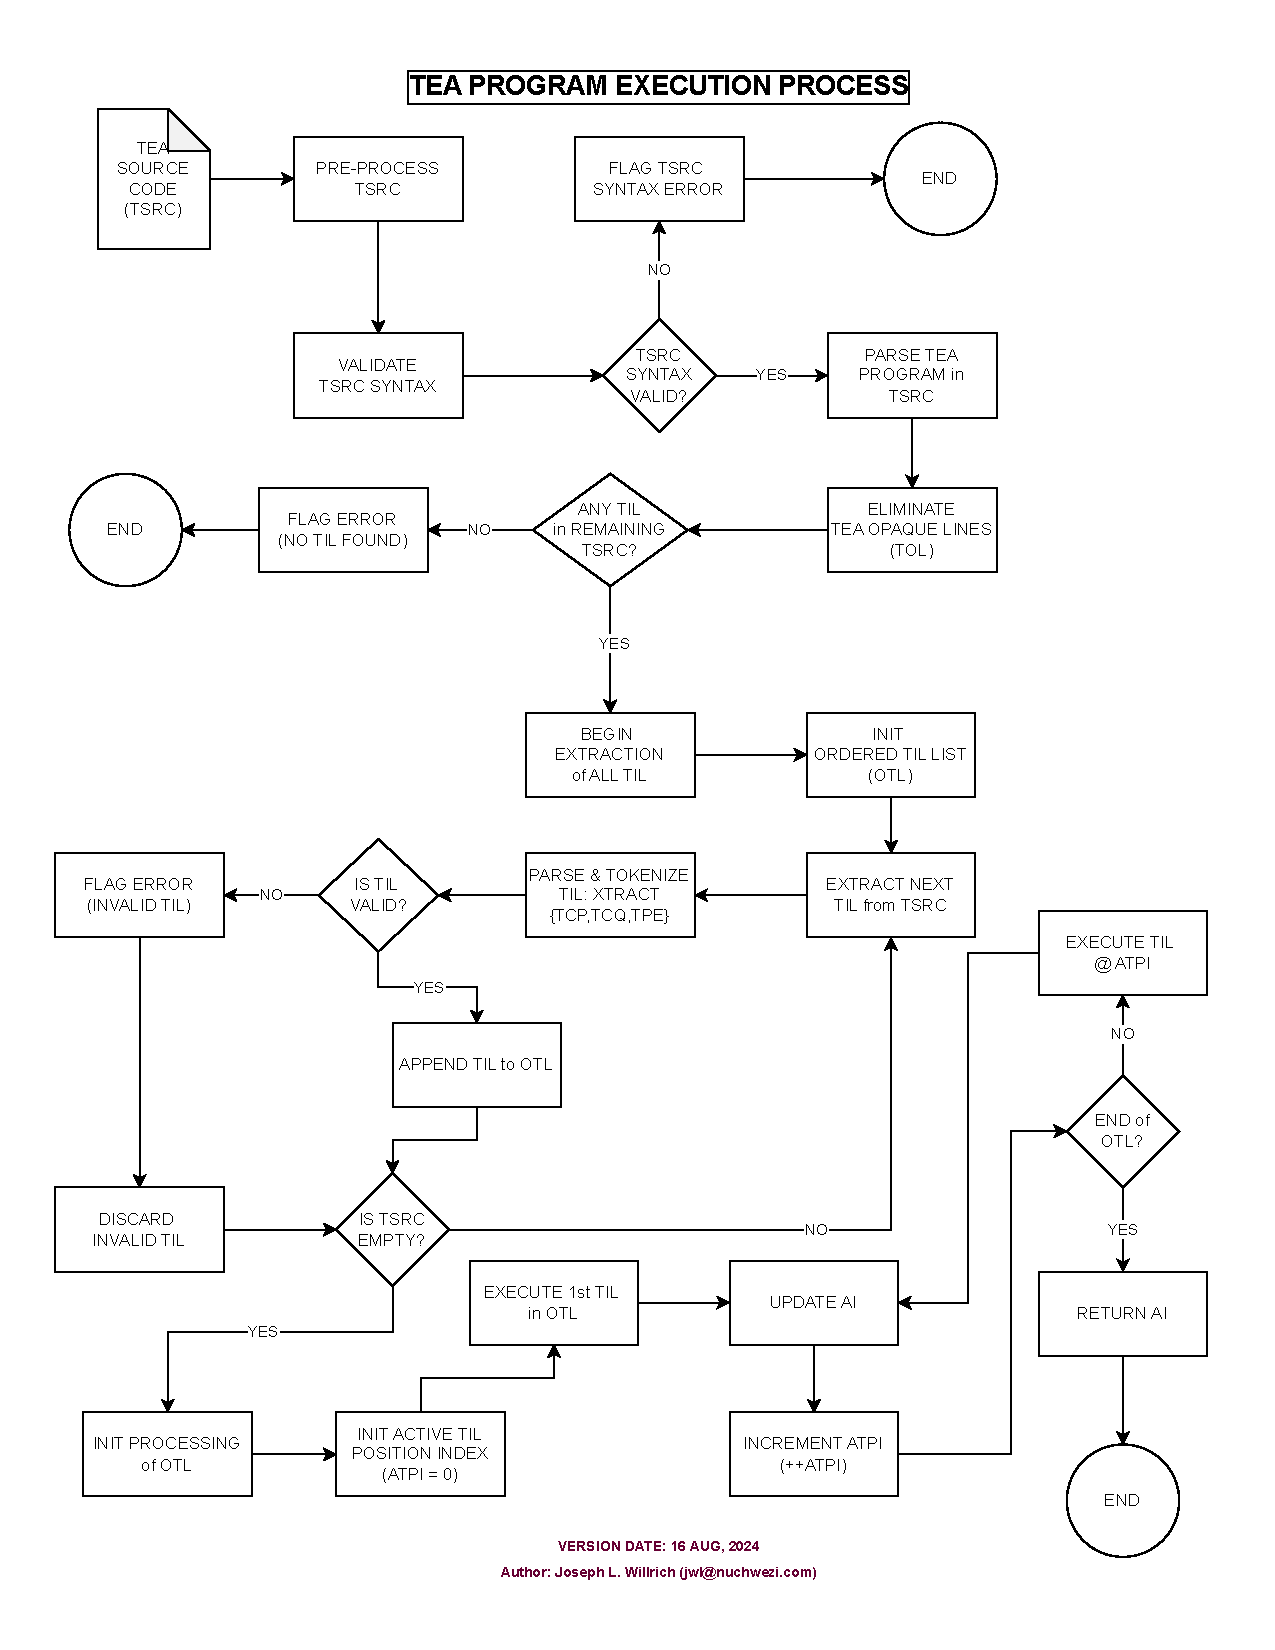
\includegraphics[trim=0cm 1cm 0cm 0cm, clip, width=0.9\textwidth,]{resources/pdfs/TEA_PROGRAM_EXEC_PROCESS.pdf}\\
   \caption{The TEA Program Execution Process.}
  \label{FIGTEAEXECPROCESS}
  \end{center}
\end{figure}


\section{Tea Instruction Set And The Tea Command Primitive Names}

First, let us look at the current reference list of the 26 TEA primitives and their formal names as depicted in \textbf{\autoref{FIGTEAISET}}:


\begin{figure}[H]
  \begin{center}
  %\includegraphics[trim=2cm 8cm 2cm 8cm, clip, width=0.9\textwidth,]{resources/pdfs/ProteinSynthesisStateMachine.pdf}\\
   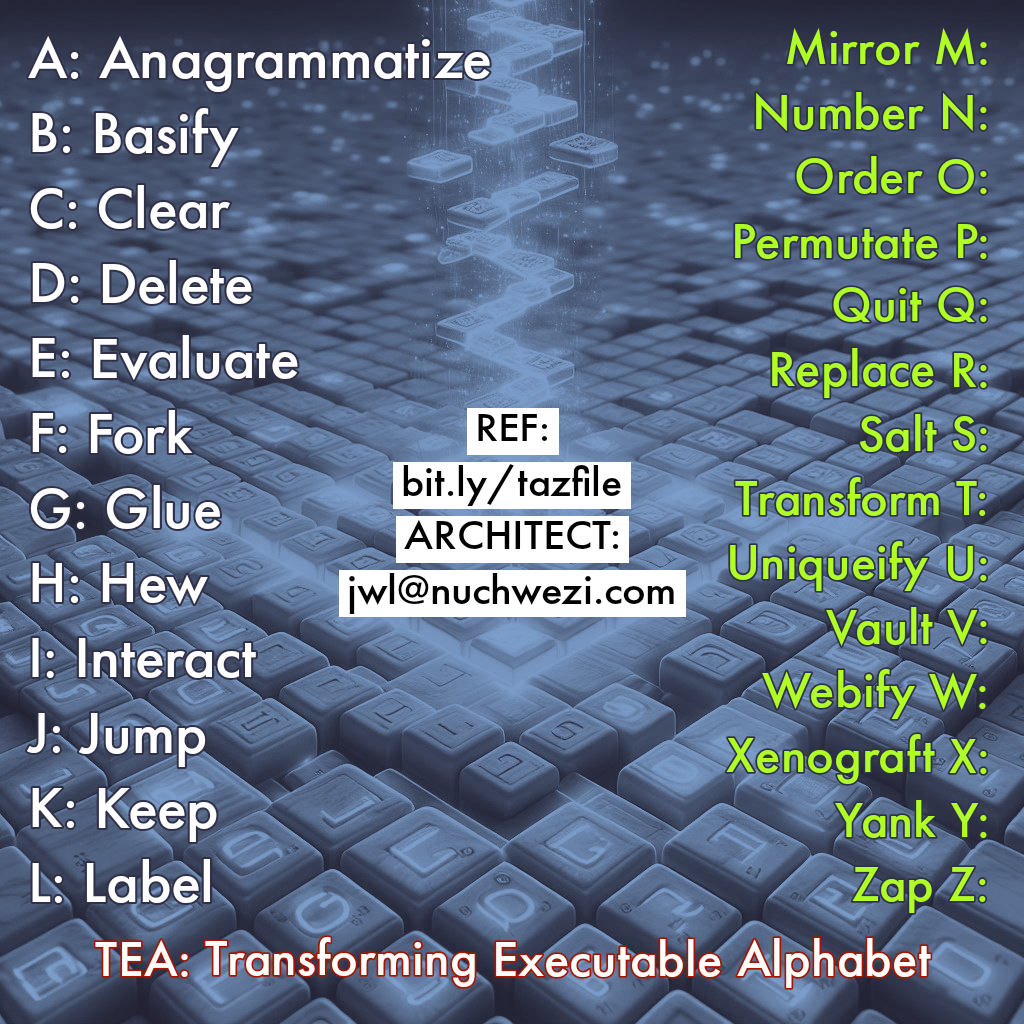
\includegraphics[trim=0cm 1cm 0cm 0cm, clip, width=0.9\textwidth,]{resources/tea_cs_is.png}\\
   \caption{The TEA Instruction Set (26 TEA Primitives and their names).}
  \label{FIGTEAISET}
  \end{center}
\end{figure}

In the rest of this manuscript, we then fully define each of these primitives, with focus on what purpose each primitive serves in a TEA program, what syntax it expects, as well as the function and semantics associated with it. For best clarity, each primitive shall be treated in its own chapter, but the approach and structure of the specification remains the same across all the 26 TEA primitives.


\subsection{The Tea Command Naming Standard}

Some people shall wonder, and correctly so, \textit{just how did we come up with the useful names for the 26 TEA primitives} as depicted in \textbf{\autoref{FIGTEAISET}}? And there is no simple answer for that except the method and creativity that the inventor of the language utilized during the architecting/design phase of the language, and so, we get a glimpse of the process that went into that task, as explained hereafter:

All TEA commands are essentially verbs - they tell the TEA processor to do something, but also, based on the name and expression of the verb, they also specify or hint at how to do that thing or what exactly to do or not do. Thus, in choosing names for the TEA Instruction Set primitive commands – which, though they might already be easy to call by the names of their constituent TEA primitive letters ``a" to ``z", would better be named suitably to distinguish them from ordinary Latin alphabet letters, and also to help reflect or clarify on their function in TEA. The following 4 guiding principles serve that purpose:


\begin{enumerate}
\item The Command Name must start with the same letter as the TEA command for which it is a name.
\item The Command Name must reflect or hint to the verb or action the command is designed to do, and not be ambiguous.
\item The Command Name must be a single word, preferably in English.
\item The Command Name must be unique across the instruction set, but this already follows from condition \#1 in this list.
\end{enumerate}

Thus, some tricky TEA primitives such as W: might perhaps better be named ``Webify" instead of original proposal to use ``Web", and for U: to be called ``Uniqueify" instead of ``Unique". But, condition \#2 somewhat helps relax or dismiss the need for these renamings if they seem too extreme. However, with the Instruction Set as expressed above, we can boldly say each of the 26 primitive instructions in TEA clearly and non-ambiguously define not only what each instruction does, but also how. Just by looking at the Command name, or even just the command's first letter... Which surely is not just a clean design choice, but also shall serve to make learning, reading and applying TEA programs very easy. Of course, unlike many of not most existing programming languages, the TEA language can boast of having the simplest instruction set, and also one that's very precise in semantics and purpose, and which, with the use of mnemonics such as reading and memorizing the TEA command name map above, becomes readily palatable and learnable even for little kids just learning the alphabet.

%%%%%%%%%%%%%%%%%%%%%%%%%%%%%%%%%%%%%%%%%%%%
% BEGIN TAZ SECTION
%%%%%%%%%%%%%%%%%%%%%%%%%%%%%%%%%%%%%%%%%%%%

\chapter{TEA A: TO Z: COMMAND SPACE SPECIFICATION (Introduction)}
\label{SECTAZ}

In the rest of this section, we shall look at the full formal specification as well as some explanatory and/or illustrative notes, as well as several example TEA programs, concerning each one of the 26 \textbf{A:} to \textbf{Z:} TEA primitives, one at a time. For historical purposes, the only other authoritative existing reference material in relation to the TAZ is in a couple of exploratory lectures\footnote{Find the \textbf{TEA: Transforming executable alphabet mini-lectures} series on YouTube: \url{https://youtube.com/playlist?list=PL9nqA7nxEPgulGKWw1L9xEyqgCdEezaKB&feature=shared}} that the language’s inventor gave mostly before this manuscript was originally prepared.

%%%%%%%%%%%%%%%%%%%%%%%%%%%%%%%%%%%%%%%%%%%%
% TAZ SECTION: A
%%%%%%%%%%%%%%%%%%%%%%%%%%%%%%%%%%%%%%%%%%%%
\chapter{A: ANAGRAMMATIZE}
\label{CHAPA}


\begin{table}[H]
  \centering
  \LARGE
	\begin{tabular}[t]{|p{0.2\textwidth}|p{0.5\textwidth}}
 
	\textbf{NAME} & Anagrammatize\\
	\hline
	\textbf{Purpose} & \begin{enumerate}
	\item Compute anagrams
	\item Shuffle lists
	\item Randomize letters
	\item Create randomness
	\end{enumerate}\\
	\hline
	              
\end{tabular}
\caption{General Objectives of A:}
  \label{TABTAZA}
\end{table}


\section{SEMANTICS of A:}
\label{SECSEMA}

\begin{table}[H]
\centering
\renewcommand{\arraystretch}{1.3} % Optional: increases row height
\rowcolors{1}{lightgray}{white}   % Alternating row colors
\begin{tabular}{>{\bfseries}m{0.3\linewidth} | m{0.6\linewidth}} % 2 columns, 

\rowcolor{white}
\textbf{\makecell[l]{INSTRUCTION\\ SIGNATURE}} & \textbf{INSTRUCTION FUNCTION} \\
\hline

a: & Set IO as the AI anagrammatized by words \\

\rowcolor{lightgray}\bfseries a:STR & Same as a:, but operating on the string STR \\

 a!: & Set IO as the AI anagrammatized by characters \\
 
\rowcolor{lightgray}\bfseries a!:STR & Same as a!:, but operating on string STR \\

 \makecell[l]{a*:vNAME \\ a*!:vNAME}& The first as a:, the second as a!:, but operating on string in vault vNAME \\
 
 \hline
\end{tabular}
\caption{The Semantics of A:}
\label{TABSEMA}
\end{table}


\section{NOTES about A:}
\label{SECNOTESA}

By the definitions above, the program:



 \begin{figure}[H]
 \Large
  \centering
  \begin{tcolorbox}[teaterminalstyle, title=TEA Program: shuffling words in a string]
  %\begin{lstlisting}[language=TEA, caption={TP A1}, label={LSTA1}, numbers=left]
  \begin{lstlisting}[language=TEA]
i!:{BC CB BA AB}|a:
   \end{lstlisting}
  \end{tcolorbox}
  %\caption{Sample TEA Program demonstrating most quirks of TEA programming (MINIFIED version)}
  %\label{FIGA1}
\end{figure}


could return “CB BA AB BC” --- note that \textbf{a:} basically shuffles the words in the AI --- which, given TEA only has the two types; regular expressions and strings, we might as well say, \textbf{a:} can shuffle words in a list (where, the items in the list are assumed to be containing no white space in them, and thus can be delimited using white space). 

On the other hand, the related but different program


 \begin{figure}[H]
 \Large
  \centering
  \begin{tcolorbox}[teaterminalstyle, title=TEA Program: shuffling a list of symbols]
  %\begin{lstlisting}[language=TEA, caption={TP A2}, label={LSTA2}, numbers=left]
  \begin{lstlisting}[language=TEA]
i!:{BC CB BA AB} | a!:
   \end{lstlisting}
  \end{tcolorbox}
  %\caption{Sample TEA Program demonstrating most quirks of TEA programming (MINIFIED version)}
  %\label{FIGA2}
\end{figure}

would return something like “  ABBCB ACB” because \textbf{a!:} shuffles the contents of the AI at character level --- it's like shuffling a list once again, but with the empty string as the delimiter this time.


\section{EXAMPLE APPLICATIONS of A:}
\label{SECEXAMPA}

Because \textbf{A:} allows us to shuffle items in a list, we might use it to construct programs that can be used to make decisions based on a random selection of some item from the list. 

\subsection{EXAMPLE 1: Randomly Pick What to Cook}
\label{SECEXAMP1A}

The following program, given a list of food items available, shall help to randomly pick what to cook on a particular day or at any moment it is tasked with making a suggestion:


 \begin{figure}[H]
 \Large
  \centering
  \begin{tcolorbox}[teaterminalstyle, title=TEA Program: randomly suggest what to cook]
  %\begin{lstlisting}[language=TEA, caption={TP A3}, label={LSTA3}, numbers=left]
  \begin{lstlisting}[language=TEA]
i!:{BURGER PIZZA OMELETTE RICE PUDDING FRIES 
MEATBALLS}|a:|d:[ ].*$|x:{I think, you make }
#(=I think, you make PUDDING, VAULTS:{})
#(=I think, you make BURGER, VAULTS:{})
   \end{lstlisting}
  \end{tcolorbox}
  \caption{TEA EXAMPLE: Random Meal Recommender}
  \label{FIGA3}
\end{figure}

Note that, like we saw in \textbf{\autoref{SECPARSE}}, the source code of a legitimate TEA program might sometimes contain non-executable lines such as TEA comments --- these being the lines shown in gray color, and which start with the character ``\#". But also, as explained in the section on how to debug TEA programs as well as in the TEA Debugging paper\cite{Lutalo2025debug}, we might sometimes want to demonstrate what is going on or what is expected to be the internal state of a TEA program at either its termination point, or anywhere before that, by placing some illustrative comments such as the last two lines in that program in \textbf{\autoref{FIGA3}}.




%%%%%%%%%%%%%%%%%%%%%%%%%%%%%%%%%%%%%%%%%%%%
% TAZ SECTION: B
%%%%%%%%%%%%%%%%%%%%%%%%%%%%%%%%%%%%%%%%%%%%
\chapter{B: BASIFY}
\label{SECB}


\begin{table}[H]
  \centering
  \LARGE
	\begin{tabular}[t]{|p{0.2\textwidth}|p{0.5\textwidth}}
 
	\textbf{NAME} & Basify\\
	\hline
	\textbf{Purpose} & \begin{enumerate}
	\item Compute the Lexical Base of input
	\item Reduce input/list to distinct symbols, sorted by their order of first occurrence in the input
	\item Reduce input to distinct symbols, sorted by their lexical/alphabetical order
	\item Implementing FIFOs
	\item Generating lexical keys
	\item Comparing things by their lexical keys
	\end{enumerate}\\
	\hline
	              
\end{tabular}
\caption{General Objectives of B:}
  \label{TABTAZB}
\end{table}


\section{SEMANTICS of B:}
\label{SECSEMB}


\begin{table}[H]
\centering
\renewcommand{\arraystretch}{1.3} % Optional: increases row height
\rowcolors{1}{lightgray}{white}   % Alternating row colors
\begin{tabular}{>{\bfseries}m{0.3\linewidth} | m{0.6\linewidth}} % 2 columns, 
\rowcolor{white}
\textbf{\makecell[l]{INSTRUCTION\\ SIGNATURE}} & \textbf{INSTRUCTION FUNCTION} \\
\hline

b: & Set IO as AI reduced to only its unique characters in their order of first occurrence within AI (\textbf{FIFO Base}) \\

\rowcolor{lightgray}\bfseries b:STR & Same as b:, but operating on string STR \\

b!: & Same as b: but with the results sorted in alphabetical order (\textbf{LEXICAL Base}) \\

\rowcolor{lightgray}\bfseries b!:STR & Same as b!: but operating on STR \\

 \makecell[l]{b*:vNAME \\ b*!:vNAME} & The first as b:, the second as b!:, but operating on string in vault vNAME \\
 
 \hline
\end{tabular}
\caption{The Semantics of B:}
\label{TABSEMB}
\end{table}


\section{NOTES about B:}
\label{SECNOTEB}

The \textbf{Lexical Base} of the AI is to be understood as the reduction of the AI to a string made of only the \textbf{unique} characters in AI, and these, then sorted in ascending \textbf{Lexical Order} for B-Inverse otherwise occurring in their order of occurrence.

By the definitions above, the program:


 \begin{figure}[H]
 \Large
  \centering
  \begin{tcolorbox}[teaterminalstyle, title=TEA Program: computing the symbol FIFO Base of AI]
  %\begin{lstlisting}[language=TEA, caption={TP B1}, label={LSTB1}, numbers=left]
  \begin{lstlisting}[language=TEA]
i!:{BC CB BA AB} | b:
   \end{lstlisting}
  \end{tcolorbox}
  %\caption{Sample TEA Program demonstrating most quirks of TEA programming (MINIFIED version)}
  %\label{FIGB1}
\end{figure}


Should return ``BC A". While  


 \begin{figure}[H]
 \Large
  \centering
  \begin{tcolorbox}[teaterminalstyle, title=TEA Program: computing LEXICAL Base of AI]
  %\begin{lstlisting}[language=TEA, caption={TP B2}, label={LSTB2}, numbers=left]
  \begin{lstlisting}[language=TEA]
i!:{bC CB BA aB} | b!:
   \end{lstlisting}
  \end{tcolorbox}
  %\caption{Sample TEA Program demonstrating most quirks of TEA programming (MINIFIED version)}
  %\label{FIGB2}
\end{figure}

Should return ``ABCab". While,  


 \begin{figure}[H]
 \Large
  \centering
  \begin{tcolorbox}[teaterminalstyle, title=TEA Program: compute FIFO Base of a literal string]
  %\begin{lstlisting}[language=TEA, caption={TP B3}, label={LSTB3}, numbers=left]
  \begin{lstlisting}[language=TEA]
b:{bC CB BA aB}
   \end{lstlisting}
  \end{tcolorbox}
  %\caption{Sample TEA Program demonstrating most quirks of TEA programming (MINIFIED version)}
  %\label{FIGB3}
\end{figure}


Shall or should return exactly ``bC BAa".

 \begin{figure}[H]
 \Large
  \centering
  \begin{tcolorbox}[teaterminalstyle, title=TEA Program: computing LEXICAL Base of data in a vault]
  %\begin{lstlisting}[language=TEA, caption={TP B4}, label={LSTB4}, numbers=left]
  \begin{lstlisting}[language=TEA]
v:vAI:{bC CB 543 12a} | b*!:vAI 
#(=12345BCab, VAULTS:{"vAI":"bC CB 543 12a"})
   \end{lstlisting}
  \end{tcolorbox}
  %\caption{Sample TEA Program demonstrating most quirks of TEA programming (MINIFIED version)}
  %\label{FIGB4}
\end{figure}

Should return ``12345BCab". 


\section{EXAMPLE APPLICATIONS of B:}
\label{SECEXAMPB}

It might be alluring to try and use \textbf{B:} to sort arbitrary things, such as attempting to sort a list of children in a classroom by their ascending birthdays in a particular month, or by the order of their first names, however, it should be worth noting that when \textbf{B:} or \textbf{B!:} process any input, they operate on it as a list of symbols or letters, and not as words --- unlike \textbf{A:}, \textbf{B:} doesn't respect white-space delimiters, and so, the best it can be used for, are cases where the sorting that needs to be done, is entirely based on order of non-compound values --- such as individual symbols, characters, digits or letters.

Thus, when passed a list such as ``10 1 9", we should not expect to get something like ``1 9 10", neither `` 0119", but shall instead get something like ``10 9" --- for ``b:" or `` 019" --- for ``b!:". These, because we are computing \textbf{bases at symbol level}.

With that clarification out of the way, we can then appreciate the following example program that can only be best implemented using \texttt{B!:}

\subsection{EXAMPLE 1: Compute Largest Possible o-SSI Number from Several Arbitrary Sequences}
\label{SECEXAMP1B}

In a paper from April 2025, fut. prof. JWL, while exploring RNGs, came across some interesting properties of certain numbers. In particular, the paper \cite{ossipaper} brought to surface the matter of numerical sequences (particularly those of decimal digits), which, when reduced to their sequence symbol set\cite{transformatics}, retain all their original member digits, but also that, those digits are exactly the same members as make-up the symbol set of the base to which the number sequence belongs --- such as $\psi_{10}$ for numbers in base-10. Such numbers, and sequences or numerical expressions of that kind, he named \textbf{orthogonal symbol set identities} (o-SSI). Of course, it is not just o-SSI sequences (meaning, a sequence $S^n: \invpi(S^n) = \invpi(\psi_{n}) = n \quad \land \quad \psi(S^n) \equiv \psi_n$) that can be reduced to an o-SSI sequence for some base-n, but any sequence, $S^k: \invpi(S^k) = k \geq \invpi(\psi_{n}) = n \quad \land \quad \psi_n(S^k) \equiv \psi_n$ also can. 

And so, a problem might arise... In case we had several arbitrary sequences of numbers --- let us assume we have n sequences, $\langle S_1, S_2, S_3,...,S_n \rangle$, each of arbitrary length, and that any two sequences from that collection might not be of the same length or cardinality, and that their member composition and distribution too might not be the same or similar, but that all these sequences span the same base symbol set --- for simplicity, assuming it is $\psi_{10}$. So, assuming we wanted to determine which of these sequences, such as some $S_m$, such that, when we reduce it to just its \textbf{natural symbol set}\footnote{Refer to \textbf{Definition 5} of \cite{ossipaper}}, and from that natural symbol set --- which might or might not be equivalent to $\psi_{10}$, further reduce it to a pure number, $P_{S_m}$. We then know as a fact, that if indeed $\invpi(\psi_{10}(S_m)) = Max(\invpi(\psi_{10}(S_i)) \forall i \in [1,n])$, then that number, if its elements are sorted in descending order of their first occurrence within $\psi_{10}$, shall be the largest possible given all such numbers we might compute for all the sequences in our collection. And further, that that number, $P_{S_m}$, shall be the largest base-10 o-SSI we can derive from the collection of sequences. Essentially that we want to perform the transformation:

\begin{trans}
\label{TRANSB1}
$\langle S_1, S_2, S_3,...,S_n \rangle \quad  \rightarrow \quad \langle P_{S_1}, P_{S_2}, P_{S_3},..., P_{S_n} \rangle  \quad \xrightarrow{O_{find\_max P_{S_i}}} P_{S_m};\\
\invpi(P_{S_m}) = m\\
\land |P_{S_m}| \geq |P_{S_i}| \quad \forall S_i, i \in [1,n]$ 
\end{trans}

And find $P_{S_m}$ given some or any such collection of sequences. Good enough, in TEA, we have the necessary tools to go about resolving such a problem, and the following basic program solves the first bit of this task: it essentially reduces any input sequence (whether purely numeric or alpha-numeric) to just its unique decimal digits (thus $\psi_{10}(S_i)$), and from that reduced sequence, to just the largest possible decimal pure number based on those digits (thus $P_{S_i}$). So, once we have a sequence of such pure numbers, of course we can determine which of them is the largest, and thus could work backwards to which sequence it was that is its source.


 \begin{figure}[H]
 \Large
  \centering
  \begin{tcolorbox}[teaterminalstyle, title=TEA Program: compute largest o-ssi from input sequence]
  %\begin{lstlisting}[language=TEA, caption={TP B5}, label={LSTB5}, numbers=left]
  \begin{lstlisting}[language=TEA]
i:{63 285 02517 abc3921 219e}
d!:[0-9]
b!: 
m!:
#(=987653210, VAULTS:{})
   \end{lstlisting}
  \end{tcolorbox}
  \caption{TEA EXAMPLE: Computing Largest o-SSI}
  \label{FIGB5}
\end{figure}

Note that in this example in \textbf{\autoref{FIGB5}}, we have wanted to demonstrate that the input sequence might contain \textit{noise} --- such as non-digit symbols, and so, these are eliminated using some of the TEA commands we shall encounter later, however, irrespective of the input, the result shall always be the largest possible decimal pure number we can form from the natural symbol set of the input under base-10.

Thus, applying this program to a set of various, random inputs as tabulated below, we see that it becomes easy to identify which of the input sequences is $S_m$.



\begin{table}[H]
  \centering
	\begin{tabular}[t]{|c|c|c|c|c|c|}
	\hline
	$i\in[1,n]$& \textbf{\makecell{INPUT:\\$S_i$}} & $S_{10}$ & $\psi_{10}(S_i)$ & $P_{S_i}$ & Rank($ \geq |P_{S_m}|$) \\
	\hline
	\makecell{Associated\\TEA} & \texttt{i:\{...\}} & \texttt{d!:[0-9]}	& \texttt{b!:} & \texttt{m!:} & \texttt{z:\{AI...\}}\\
	\hline
	\hline	
	1&$\langle 63 285 02517 abc3921 219e \rangle$ & $\langle 63 285 02517 abc3921 219e \rangle$ & 012356789 & 987653210 & 1\\
	\hline
	2&$\langle 63 25 02517 \rangle$ & $\langle 632502517 \rangle$  & 0123567 & 7653210 & 2\\
	\hline
	3&$\langle 1998 1994 1984 1001 \rangle$ & $\langle 1998199419841001 \rangle$ & 01489 & 98410  & 4\\
	\hline
	4&$\langle 124 999 452 111 98 ae this is 9519 \rangle$ & $\langle 124999452111989519 \rangle$ & 124589  & 985421 & 3\\
	\hline	              
\end{tabular}
  \caption{Tabular Analysis to identify $S_m$ given a collection of arbitrary alpha-numeric sequences}
    \label{TABANAB1}
\end{table}


From the analysis we have conducted in \textbf{\autoref{TABANAB1}}, and which is based on computations we conduct on the input/presented data --- alpha-numeric sequences $S_{i\in [1,n]}$, as depicted in the TEA program (see  \textbf{\autoref{FIGB5}}), we find that the solution to our problem then, shall be the sequence:

\begin{equation}
\label{EQB1}
S_1 = \langle 63 285 02517 abc3921 219e \rangle
\end{equation}

And how did we know or how might we prove this? Or rather, how did we arrive at the final results in the \textbf{RANK} column? Without evolving the original program further, note that, once we have the $P_{S_i}$ values ($5^{th}$ column), we then can sort them --- not lexically as usual TEA might allow, but numerically, and with use of some little \textit{external power} as we shall see when we come to the TEA primitive \textbf{Z:}:



 \begin{figure}[H]
 \Large
  \centering
  \begin{tcolorbox}[teaterminalstyle, title=TEA Program: sort in descending order numbers from input sequence]
  %\begin{lstlisting}[language=TEA, caption={TP B6}, label={LSTB6}, numbers=left]
  \begin{lstlisting}[language=TEA]
i:{987653210 7653210 98410 985421} 
r!:[ ]+:,
x:[
x!:]
z:{JSON.parse(AI).map(s=>Number(s)).sort((a,b)=>b-a)}
h!:,
d:,
   \end{lstlisting}
  \end{tcolorbox}
  \caption{TEA EXAMPLE: Numerically Sorting Words/Values/Numbers in TEA}
  \label{FIGB6}
\end{figure}


And when we run that program depicted in \textbf{\autoref{FIGB6}}, we obtain the following output:


\begin{figure}[H]
  \centering
  \begin{tcolorbox}[myterminalstyle, title=TEA Output from \textbf{\autoref{FIGB6}}]
  \begin{lstlisting}
987653210
7653210
985421
98410
  \end{lstlisting}
  \end{tcolorbox}
  \caption{Result of numerically sorting numeric projections}
\end{figure}

Which then gives us the rankings, and from that we determine the solution to our original problem. Thus we conclude our treatment of \textbf{B:} for now.


%%%%%%%%%%%%%%%%%%%%%%%%%%%%%%%%%%%%%%%%%%%%
% TAZ SECTION: C
%%%%%%%%%%%%%%%%%%%%%%%%%%%%%%%%%%%%%%%%%%%%
\chapter{C: CLEAR}
\label{CHAPC}


\begin{table}[H]
  \centering
  \LARGE
	\begin{tabular}[t]{|p{0.2\textwidth}|p{0.5\textwidth}}
 
	\textbf{NAME} & Clear\\
	\hline
	\textbf{Purpose} & \begin{enumerate}
	\item Clear working memory
	\item Reset all vaults (TEA variables in memory)
	\item Reset particular/named vaults
	\item Reset AI
	\item Guarantee subsequent instructions set memory independently of earlier instructions
	\item Automagically create and initialize named vaults with the EMPTY STRING value.
	\end{enumerate}\\
	\hline
	              
\end{tabular}
\caption{General Objectives of C:}
  \label{TABTAZC}
\end{table}


\section{SEMANTICS of C:}
\label{SECSEMC}

\begin{table}[H]
\centering
\renewcommand{\arraystretch}{1.3} % Optional: increases row height
\rowcolors{1}{lightgray}{white}   % Alternating row colors
\begin{tabular}{>{\bfseries}m{0.3\linewidth} | m{0.6\linewidth}} % 2 columns, 

\rowcolor{white}
\textbf{\makecell[l]{INSTRUCTION\\ SIGNATURE}} & \textbf{INSTRUCTION FUNCTION} \\
\hline

c: & Set Empty String as IO/AI \\

\rowcolor{lightgray}\bfseries c:PARAMS & INERT \\

 c!: & Set Empty String as IO and set to Empty String all 
currently active vaults (including the DEFAULT VAULT)\\
 
\rowcolor{lightgray}\bfseries c!:PARAMS & INERT\\

 c*: & INERT\\
 
 \rowcolor{lightgray}\bfseries \makecell[l]{c*:v1:v2:…:vN \\ c*!:v1:v2:…:vN}& \textbf{ONLY} clear/reset the vaults specified by the given vault names v1, v2,…, vN. Does NOT tamper with IO/AI. \textbf{INCASE} any of the specified vault names points to a vault that does not yet exist, then it shall be created, and automatically initialized with the EMPTY STRING.\\
 
 \hline
\end{tabular}
\caption{The Semantics of C:}
\label{TABSEMC}
\end{table}


\section{NOTES about C:}
\label{SECNOTESC}

For especially purposes of \textbf{C:}, note that the \textbf{Empty String} is the sequence “” --- essentially, a string of 0 length, and that, by setting some vault or variable to that value, we effectively deem it ``reset" or ``cleared". The \textbf{C:} commands DO NOT declare nor [re-]write new or previously undeclared memory spaces --- vaults to be precise, but rather, modify existing, named (and in the case of \texttt{c:}, also the \texttt{DEFAULT/UNNAMED VAULT}\footnote{In TEA parlance, the ``Unnamed" or ``Default Vault" does come up several times as you shall see when exploring the TAZ, and it plays a very crucial role in TEA programming as we shall also come to learn. But essentially, it is a vault whose name is just the EMPTY STRING, ``". Typically, only special instructions can create such a vault, and users of vault-creating primitives such as \texttt{v:vNAME} can not directly create or write to it using an empty name. More about this later.}\footnote{Talking of globally resetting working memory in a TEA program, using say \texttt{c!:}, it shall be useful or rather important to note that, there is JUST ONE variable that no \textbf{C:} command can clear or reset, and that is the \textbf{Initial AI} --- the external, user-provided input at the start of a TEA program is always, and shall always (if it was indeed provided), remain accessible via a special TEA instruction known as \textbf{Yank}; particularly, the instruction \texttt{y*:}, which we shall formally cover in the chapter on \textbf{Y:}.}


With that introduction and the formal specifications of \textbf{C:} out of the way, the program:


 \begin{figure}[H]
 \Large
  \centering
  \begin{tcolorbox}[teaterminalstyle, title=TEA Program: resetting explicitly set AI]
    %\begin{lstlisting}[language=TEA]
  \begin{lstlisting}[language=TEA, caption={TP C1}, label={LSTC1}, numbers=left]
i!:{BC}| c:
# (=, VAULTS:{})
   \end{lstlisting}
  \end{tcolorbox}
  %\caption{Sample TEA Program demonstrating most quirks of TEA programming (MINIFIED version)}
  %\label{FIGC1}
\end{figure}

Despite having an explicit, hard-coded input specified in the first instruction of the program as ``BC", shall, and should return just ``" as expected. While  


\begin{figure}[H]
 \Large
  \centering
  \begin{tcolorbox}[teaterminalstyle, title=TEA Program: \texttt{c:} does not clear DEFAULT VAULT]
    %\begin{lstlisting}[language=TEA]
  \begin{lstlisting}[language=TEA, caption={TP C2}, label={LSTC2}, numbers=left]
i!:{BC} | v: | c: | y:
# (=BC, VAULTS:{"":"BC"})
   \end{lstlisting}
  \end{tcolorbox}
  %\caption{Sample TEA Program demonstrating most quirks of TEA programming (MINIFIED version)}
  %\label{FIGC2}
\end{figure}

Should return ``BC". The main difference between those two programs --- which actually initialize their initial input/AI in the same exact way, is that, for the case in \textbf{\autoref{LSTC1}}, \texttt{c:} is invoked before any chance is given to stash the AI somewhere for later use, while, as we see in \textbf{\autoref{LSTC2}}, we first store the input into some memory location --- with \texttt{v:} in this case, which, as we shall see in the section on \textbf{V:}, writes AI to the \textbf{DEFAULT VAULT}, so that, by the time we call \texttt{c:}, which ONLY resets AI, we have that value still accessible later, when we invoke the vault-reading instruction \texttt{y:}\footnote{Concerning this example, note that indeed, as shown in the commented out line, which dumps the state of the TEA runtime at the moment the program exits, we see that indeed, the Default Vault held the stashed value of the original AI so that we can still be able to later read it unless say \texttt{c!:} had been invoked somewhere before termination of the program.}.

However, in the next example:


\begin{figure}[H]
 \Large
  \centering
  \begin{tcolorbox}[teaterminalstyle, title=TEA Program: \texttt{c!:} resets all memory]
    %\begin{lstlisting}[language=TEA]
  \begin{lstlisting}[language=TEA, caption={TP C3}, label={LSTC3}, numbers=left]
i!:{BC} | v: | v:XX:{T} | c!: | y:XX
# (=, VAULTS:{"":"","XX":""})
   \end{lstlisting}
  \end{tcolorbox}
  %\caption{Sample TEA Program demonstrating most quirks of TEA programming (MINIFIED version)}
  %\label{FIGC3}
\end{figure}


We note that we shall still end up with the result ``" because whether or not we read the main/implicit memory (AI) or any explicit/named memory (such as the default vault via \texttt{y:} or the ``XX” vault written to in this example program, and which we later read using \texttt{y:XX}), after a call to c!:, all active memory is essentially cleared --- as seen in the dump of the final runtime state in the last comment of \textbf{\autoref{LSTC3}}.


For cases where one wishes to clear only specific sections of memory, via named vaults, the following example can be illustrative enough:

\begin{figure}[H]
 \Large
  \centering
  \begin{tcolorbox}[teaterminalstyle, title=TEA Program: \texttt{c!:} resets all memory]
    %\begin{lstlisting}[language=TEA]
  \begin{lstlisting}[language=TEA, caption={TP C4}, label={LSTC4}, numbers=left]
i!:{BC} | v: | c: | y: | a!: |
v:vA | n:100 | v:vB | v:vGLUE:** 
| c*!:vA | g*!:vGLUE:vA:vB
   \end{lstlisting}
  \end{tcolorbox}
  %\caption{Sample TEA Program demonstrating most quirks of TEA programming (MINIFIED version)}
  %\label{FIGC4}
\end{figure}

That program should return ``**N" where N is some random number (e.g ``BC**98"). Otherwise, without \texttt{c*!:vA}, such as in the following version:

\begin{figure}[H]
 \Large
  \centering
  \begin{tcolorbox}[teaterminalstyle, title=TEA Program: \texttt{c!:} resets all memory]
    %\begin{lstlisting}[language=TEA]
  \begin{lstlisting}[language=TEA, caption={TP C5}, label={LSTC5}, numbers=left]
i!:{BC} | v: | c: | y: | a!: | 
v:vA | n:100 | v:vB | v:vGLUE:** 
| g*!:vGLUE:vA:vB
   \end{lstlisting}
  \end{tcolorbox}
  %\caption{Sample TEA Program demonstrating most quirks of TEA programming (MINIFIED version)}
  %\label{FIGC4}
\end{figure}

 
 should return something like ``CB**N" or ``BC**N" (e.g ``CB**42") because nothing reset or cleared the associated memory space, \texttt{vA}. 
 
 One would get an appreciation of how these commands work, by inspecting the resultant system state at the end of running that earlier program in \textbf{\autoref{LSTC4}} as shown in the following TEA Debugger output and memory dump associated with running that program\footnote{Shown here in two separate screenshots, because of the length of the total output.} Vs running the second/modifed program in \textbf{\autoref{LSTC5}}.
 
 
 \begin{figure}[H]
  \centering
  \begin{tcolorbox}[myterminalstyle, title=Truncated TEA Debugger Output from executing \textbf{\autoref{LSTC4}}]
  \begin{lstlisting}
No explicit INPUT found
INPUT:
 
CODE:
 i!:{BC} | v: | c: | y: | a!: |
v:vA | n:100 | v:vB | v:vGLUE:** 
| c*!:vA | g*!:vGLUE:vA:vB
---------[ IN TEA RUNTIME ]

+++[NO TEA CODE ERRORS FOUND YET]
#13 of ["i!:{BC} "," v: "," c: "," y: "," a!: ","","v:vA "," n:100 "," v:vB "," v:vGLUE:** ",""," c*!:vA "," g*!:vGLUE:vA:vB"]
CLEAN TEA CODE TO PROCESS:
i!:{BC} 
v: 
c: 
.
.
.
--[#11 TEA INSTRUCTIONS FOUND]---
...
Processing Instruction: c: 
PRIOR MEMORY STATE: (=BC, VAULTS:{"":"BC"})
RESULTANT MEMORY STATE: (=, VAULTS:{"":"BC"})
Executing Instruction#3 (out of 11)
Processing Instruction: y: 
PRIOR MEMORY STATE: (=, VAULTS:{"":"BC"})
+++[WARNING] INSTRUCTION WITH NO DATA TO PROCESS FOUND: y: 
--[INFO] Reading VAULT[]
[INFO] Returning string  in DEFAULT VAULT [BC]
RESULTANT MEMORY STATE: (=BC, VAULTS:{"":"BC"})
Executing Instruction#4 (out of 11)
Processing Instruction: a!: 
PRIOR MEMORY STATE: (=BC, VAULTS:{"":"BC"})
RESULTANT MEMORY STATE: (=CB, VAULTS:{"":"BC"})
Executing Instruction#5 (out of 11)
Processing Instruction: v:vA 
PRIOR MEMORY STATE: (=CB, VAULTS:{"":"BC"})
--[INFO] Wrote VAULT[vA = [CB]]
RESULTANT MEMORY STATE: (=CB, VAULTS:{"":"BC","vA":"CB"})
Executing Instruction#6 (out of 11)
Processing Instruction: n:100 
PRIOR MEMORY STATE: (=CB, VAULTS:{"":"BC","vA":"CB"})
RESULTANT MEMORY STATE: (=95, VAULTS:{"":"BC","vA":"CB"})
... 
PRIOR MEMORY STATE: (=95, VAULTS:{"":"BC","vA":"CB","vB":"95"})
--[INFO] Wrote VAULT[vGLUE = [**]]
RESULTANT MEMORY STATE: (=95, VAULTS:{"":"BC","vA":"CB","vB":"95","vGLUE":"**"})
Executing Instruction#9 (out of 11)
Processing Instruction: c*!:vA 
PRIOR MEMORY STATE: (=95, VAULTS:{"":"BC","vA":"CB","vB":"95","vGLUE":"**"})
RESULTANT MEMORY STATE: (=95, VAULTS:{"":"BC","vA":"","vB":"95","vGLUE":"**"})
Executing Instruction#10 (out of 11)
Processing Instruction: g*!:vGLUE:vA:vB
PRIOR MEMORY STATE: (=95, VAULTS:{"":"BC","vA":"","vB":"95","vGLUE":"**"})
--[INFO] Reading VAULT[vGLUE]
--[INFO] Reading VAULT[vA]
--[INFO] Reading VAULT[vB]
RESULTANT MEMORY STATE: (=**95, VAULTS:{"":"BC","vA":"","vB":"95","vGLUE":"**"})
  \end{lstlisting}
  \end{tcolorbox}
  \caption{TEA Debugger Output for Understanding Memory Alteration via \texttt{c*!:vA}}
  \label{FIGC5}
\end{figure}


\begin{figure}[H]
  \centering
  \begin{tcolorbox}[myterminalstyle, title=Truncated TEA Debugger Output from executing \textbf{\autoref{LSTC5}}]
  \begin{lstlisting}
...
---------[ IN TEA RUNTIME ]

+++[NO TEA CODE ERRORS FOUND YET]
#12 of ["i!:{BC} "," v: "," c: "," y: "," a!: "," ","v:vA "," n:100 "," v:vB "," v:vGLUE:** ",""," g*!:vGLUE:vA:vB"]
CLEAN TEA CODE TO PROCESS:
i!:{BC} 
v: 
c: 
y: 
a!: 
v:vA 
n:100 
v:vB 
v:vGLUE:** 
g*!:vGLUE:vA:vB
--[#10 TEA INSTRUCTIONS FOUND]---
...
Processing Instruction: y: 
PRIOR MEMORY STATE: (=, VAULTS:{"":"BC"})
+++[WARNING] INSTRUCTION WITH NO DATA TO PROCESS FOUND: y: 
--[INFO] Reading VAULT[]
[INFO] Returning string  in DEFAULT VAULT [BC]
RESULTANT MEMORY STATE: (=BC, VAULTS:{"":"BC"})
Executing Instruction#4 (out of 10)
Processing Instruction: a!: 
PRIOR MEMORY STATE: (=BC, VAULTS:{"":"BC"})
RESULTANT MEMORY STATE: (=CB, VAULTS:{"":"BC"})
Executing Instruction#5 (out of 10)
Processing Instruction: v:vA 
PRIOR MEMORY STATE: (=CB, VAULTS:{"":"BC"})
--[INFO] Wrote VAULT[vA = [CB]]
RESULTANT MEMORY STATE: (=CB, VAULTS:{"":"BC","vA":"CB"})
Executing Instruction#6 (out of 10)
Processing Instruction: n:100 
PRIOR MEMORY STATE: (=CB, VAULTS:{"":"BC","vA":"CB"})
RESULTANT MEMORY STATE: (=81, VAULTS:{"":"BC","vA":"CB"})
Executing Instruction#7 (out of 10)
Processing Instruction: v:vB 
PRIOR MEMORY STATE: (=81, VAULTS:{"":"BC","vA":"CB"})
--[INFO] Wrote VAULT[vB = [81]]
RESULTANT MEMORY STATE: (=81, VAULTS:{"":"BC","vA":"CB","vB":"81"})
Executing Instruction#8 (out of 10)
Processing Instruction: v:vGLUE:** 
PRIOR MEMORY STATE: (=81, VAULTS:{"":"BC","vA":"CB","vB":"81"})
--[INFO] Wrote VAULT[vGLUE = [**]]
RESULTANT MEMORY STATE: (=81, VAULTS:{"":"BC","vA":"CB","vB":"81","vGLUE":"**"})
Executing Instruction#9 (out of 10)
Processing Instruction: g*!:vGLUE:vA:vB
PRIOR MEMORY STATE: (=81, VAULTS:{"":"BC","vA":"CB","vB":"81","vGLUE":"**"})
--[INFO] Reading VAULT[vGLUE]
--[INFO] Reading VAULT[vA]
--[INFO] Reading VAULT[vB]
RESULTANT MEMORY STATE: (=CB**81, VAULTS:{"":"BC","vA":"CB","vB":"81","vGLUE":"**"})
  \end{lstlisting}
  \end{tcolorbox}
  \caption{TEA Debugger Output for Understanding Memory Alteration via C:}
  \label{FIGC6}
\end{figure}

Before we close the discussion about \texttt{C:}, note that, if the vault-manipulating variants of the \textbf{CLEAR} TEA primitve are invoked with names to vaults that don't yet exist, then they shall automatically create those vaults without complaining, and initialize them to ``". 

An illustration of this effect is demonstrated when we invoke the program:


\begin{figure}[H]
 \Large
  \centering
  \begin{tcolorbox}[teaterminalstyle, title=TEA Program: explore selective processing of vaults by c*]
  %\begin{lstlisting}[language=TEA, caption={TP C6}, label={LSTC6}, numbers=left]
    \begin{lstlisting}[language=TEA]
v:vC:TEST|v:vF:TEST-F|c*!:vC:vD
   \end{lstlisting}
  \end{tcolorbox}
  %\caption{Sample TEA Program demonstrating most quirks of TEA programming (MINIFIED version)}
  %\label{FIGC6}
\end{figure}


On the TEA commandline as shown in the following screenshot:

\begin{figure}[H]
  \centering
  \begin{tcolorbox}[myterminalstyle, title=Selective Processing of Vaults by \texttt{C*:} and \texttt{C*!:}]
  \begin{lstlisting}
EXPERIMENTS|< 15:22:41 $>* tttt -c "v:vC:TEST|v:vF:TEST-F|c*!:vC:vD" -d
No explicit INPUT found, using STDIN!
INPUT:
 None
CODE:
 v:vC:TEST|v:vF:TEST-F|c*!:vC:vD
---------[ IN TEA RUNTIME ]

+++[NO TEA CODE ERRORS FOUND YET]
CLEAN TEA CODE TO PROCESS:
v:vC:TEST
v:vF:TEST-F
c*!:vC:vD
--[#3 TEA INSTRUCTIONS FOUND]---

---<< EXTRACTED TEA LABEL BLOCKS:
{}

Executing Instruction#0 (out of 3)
Processing Instruction: v:vC:TEST
PRIOR MEMORY STATE: (=, VAULTS:{})
-- [INFO] Wrote VAULT[vC = [TEST]]
RESULTANT MEMORY STATE: (=, VAULTS:{'vC': 'TEST'})
Executing Instruction#1 (out of 3)
Processing Instruction: v:vF:TEST-F
PRIOR MEMORY STATE: (=, VAULTS:{'vC': 'TEST'})
-- [INFO] Wrote VAULT[vF = [TEST-F]]
RESULTANT MEMORY STATE: (=, VAULTS:{'vC': 'TEST', 'vF': 'TEST-F'})
Executing Instruction#2 (out of 3)
Processing Instruction: c*!:vC:vD
PRIOR MEMORY STATE: (=, VAULTS:{'vC': 'TEST', 'vF': 'TEST-F'})
RESULTANT MEMORY STATE: (=, VAULTS:{'vC': '', 'vF': 'TEST-F', 'vD': ''})
  \end{lstlisting}
  \end{tcolorbox}
  \caption{TEA Debugger Output for Understanding Selective Processing of Vaults by \texttt{C*:} and \texttt{C*!:}}
  \label{FIGC7}
\end{figure}


\section{EXAMPLE APPLICATIONS of C:}
\label{SECEXAMPC}

\texttt{C:} is mostly about clearing or rather, managing memory. Quite an important facility for those who recall the ancient days of programming in languages such as C and C++, that not only made available the nifty and useful, but also painful facility of pointers and manual memory management! Luckily, in TEA, the programmer need not worry much about manual management of memory --- particularly, with regards to correctly creating, initializing and clearing or especially disposing of/returning memory to the system, because much of it is already catered for by the TEA runtime, and no possibility for example, exists, for a TEA program to directly or readily write uninitialized memory, nor for the program to quit without correctly returning memory to the underlying system.

However, that said, and given the only way to use memory with references or pointers is via TEA Vaults, we then shall acknowledge and appreciate, that, with proper use of the basic facility to create, set, update and clear memory\footnote{\textbf{WARNING:} note that, currently (as of \textbf{TEA v1.1.0} --- see \url{https://tea.nuchwezi.com} for latest), TEA provides no direct means to delete entirely or rather, to unregister a previously named memory pointer/variable reference such as with vault names, other than merely clearing the referenced memory space (such as by setting it to the EMPTY SPACE). But if required, perhaps future TEA versions might avail this functionality as a subset of \textbf{C*:} or \textbf{C.:} command space.}, the software programmer can design or implement many useful and efficient computer programs that might leverage logic that relies on the state of the program's memory so as to perform correctly. The following non-trivial, but still basic program, is a great illustration of such a computer program.


\subsection{EXAMPLE 1: The N-SIGIL Generator: print visual qrcode corresponding to some number N}
\label{SECEXAMP1C}

This program we are going to look at next, is mostly classified as both a graphical and interactive game-like software that can correctly work as written, for particularly WEB TEA\footnote{As we have indicated in \textbf{\autoref{SEC1}}, programs leveraging the \texttt{Z:CMD} instructions might not be readily portable across just WEB and CLI TEA.} --- access to which is currently readily possible via the \textbf{TEA WEB Integrated Development Environment}: \url{https://tea.nuchwezi.com}.

The program was originally developed to be part of the standard demonstration programs for the WEB TEA suite, and at basic, it does the following:

\begin{enumerate}
\item Given some numeric input, $n$, that lies within some pre-configured range: $1 \leq n \leq (nCols \times nRows)$, shall proceed to process that user-provided response, $n$, so that it then prints a matrix of $(nCols \times nRows)$ on the screen, and inside which it plots and prints a specific and deterministic basic diagram mapping the specified argument to some finite number of ``graphical bits" that unlike the rest of the matrix or grid, are \textbf{ON}, while the rest are \textbf{OFF}.
\item Essentially, it prints a ``sigil" or rather a kind of ``QRCode" or primitive ``Barcode" that can uniquely distinguish the provided number argument from any other\footnote{No, currently, it is not guaranteed to always return a universally distinct sigil for any real number, given some  numbers might result in a projection that is shared by other numbers too, but, for a particular set of $(nCols \times nRows)$, any particular $n$ is guaranteed to result in the same projection or picture across invocations of the same program or algorithm.}.
\item After prompting for and displaying the image corresponding to a user provided response, the program first clears the core graphics memmory previously utilized, via leveraging the TEA \texttt{c*:vNAME} instructions, and then re-iterates, prompting the user for the next number to visualize.
\item It is written to be intelligent enough despite its text-only user-interface, so that, once the user feels like quitting or stopping, they can just respond with the \textbf{STOP}-command; ``end", and then the program shall quit.
\end{enumerate}

In a somewhat verbose style --- so that TEA-newcomers might also get the chance to see what non-trivial TEA programming is like, as well as learn some useful quirks of how to jaggle things in TEA, we shall intermix code and comments, as well as mostly use the unminified style of TEA source.


 %\begin{figure}[H]
 \small
  \centering
  \begin{tcolorbox}[teaterminalstyle, title=TEA Program: N-SIGIL image generator program, breakable]
  %\begin{lstlisting}[language=TEA, caption={TP C7}, label={LSTC7}, numbers=left]
  \begin{lstlisting}[language=TEA,breaklines=true]
#~~[WELCOME to N-SIGIL v1.0.0]
#~~[not for the faint of heart]
#--|original algorithm by fut.prof. JWL
#--|WARNING: this TEA program is meant to 
#--|work as currently implemented
#--|ONLY for WEB TEA such as: 
#--| https://tea.nuchwezi.com
#----------------------------------------------------|

#BEGIN: determine what our image dimensions 
# shall be (not user-set)
v:vCOL:6 #columns
v:vROW:6 #rows
g*:*:vCOL:vROW | v:vN | z*:vN | v:vN #cardinality of grid (=20)

l:lSTART
#first, CLEAR/INIT key vaults:
c*!:vA:vAA:vB:vC:vD:vE:vF

i!:{=======[WELCOME to N-SIGILS]======
N-SIGILS v.1.0.0 is written in TEA v.1.1.0, 
and is an experiment to do basic graphics 
in TEA using text-processing. It is entertaining,
and will help you draw a basic QR-CODE sigil
for any number you specify. It is also interactive;
At any moment, you can quit if you like.
=============================}|i: #instructions

i!:{Preferably, pick a number between 1 and } 
| x*!:vN | x!:{ }|x!: (or `end' to QUIT): | v:vPROMPT
i: #prompt
v:vRESPONSE # stash user response
#store marshalled answer (e.g vANS=8)
z:{Math.abs(Number(AI))||1} | v:vANS 

#otherwise, first confirm if we got a legit number
y:vRESPONSE # retrieve user response
z:{Number(AI)} 
f!:NaN:lPROCESS_BLANK
j:lERRORNaN 

#check we are processing a blank number
l:lPROCESS_BLANK
y:vRESPONSE
f!:^$:lPROCESS
j:lERRORNaN

#continue to process
l:lPROCESS

y:vANS #retrieve number we saved

#compute vA
#adjust as: ((n)=>Math.floor(n/vN) + (n%vN))(vA)
v:vEXP1:((n)=>Math.floor(n/|
v:vEXP2:) + (n%|v:vEXP3:))(|v:vEXP4:)
v:vA | g*:{}:vEXP1:vN:vEXP2:vN:vEXP3:vA:vEXP4 |
v:vCMDA|z*:vCMDA|v:vA #vA=8

#compute vAA
#adjust as: ((n)=>(Math.floor(n/vCOL) + (n%vCOL))%vCOL)(vA)
v:vEXP1:((n)=>(Math.floor(n/|v:vEXP2:) + (n%|
v:vEXP3:))%|v:vEXP4:)(|v:vEXP5:)
| g*:{}:vEXP1:vCOL:vEXP2:vCOL:vEXP3:vCOL:vEXP4:vA:vEXP5 
|v:vCMDAA|z*:vCMDAA|v:vAA #vAA=4
 
#vA -> compute vB: ((n)=>(vN + n)%vCOL)(vA)
v:vEXP1:((n)=>(|v:vEXP2: + n)%|v:vEXP3:)(|v:vEXP4:)
g*:{}:vEXP1:vN:vEXP2:vCOL:vEXP3:vA:vEXP4 |v:vCMDB|
z*:vCMDB|v:vB #vB=3

#vB -> compute vC: ((n)=>Math.abs(vN - n)%vCOL)(vB)
v:vEXP1:((n)=>Math.abs(|v:vEXP2: - n)%|v:vEXP3:)(|v:vEXP4:)
g*:{}:vEXP1:vN:vEXP2:vCOL:vEXP3:vB:vEXP4 |v:vCMDC|
z*:vCMDC|v:vC #vC=2

#vC -> compute vD: 
#((n)=>Math.floor((n*vN*0.5)/vROW) + Math.floor((n*vN*0.5)%vROW))(vC)
v:vEXP1:((n)=>Math.floor((n*|v:vEXP2:*0.5)/|
v:vEXP3:) + Math.floor((n*|v:vEXP4:*0.5)%|v:vEXP5:))(|v:vEXP6:)
g*:{}:vEXP1:vN:vEXP2:vROW:vEXP3:vN:vEXP4:vROW:vEXP5:vC:vEXP6 |
v:vCMDD|z*:vCMDD|v:vD #vD=5

#vD -> compute vE: 
#((n)=>Math.floor(Math.abs(n - vN*0.5)/vROW) 
#+ Math.floor(Math.abs(n - vN*0.5)%vROW))(vD)
v:vEXP1:((n)=>Math.floor(Math.abs(n - |v:vEXP2:*0.5)/|
v:vEXP3:) + Math.floor(Math.abs(n - |v:vEXP4:*0.5)%|v:vEXP5:))(|v:vEXP6:)
g*:{}:vEXP1:vN:vEXP2:vROW:vEXP3:vN:vEXP4:vROW:vEXP5:vD:vEXP6 
|v:vCMDE|z*:vCMDE|v:vE #vE=2

#vD -> compute vF: 
#((n)=>Math.floor(Math.abs(n*0.5)/vCOL) + Math.floor(Math.abs(n*0.5)%vCOL))(vN)
v:vEXP1:((n)=>Math.floor(Math.abs(n*0.5)/|
v:vEXP2:) + Math.floor(Math.abs(n*0.5)%|v:vEXP3:))(|v:vEXP4:)
g*:{}:vEXP1:vCOL:vEXP2:vCOL:vEXP3:vN:vEXP4 |
v:vCMDF|z*:vCMDF|v:vF #vF=5

#DEBUG: show which coordinates to shade
#1: vA -> (1,vAA) -> (1,4)
#2: vB -> (2,vB) -> (2,3)
#3: vC -> (3,vC) -> (3,2)
#5: vD -> (4,vD) -> (4,5)
#6: vE -> (vF, vE) -> (5,2)

#Given vCOL x vROW -> (5x4) and <(x,y)*> simulate...
###X#
##X##
#X###
#X###

#----[presenting results]-------
l:RESULT

#first, construct the specification for the grid to print
#vCOORDINATES=[(1,vAA), (2,vB), (3,vC), (4,vD),(vF, vE)]
#v:vEXP1:[(1,|v:vEXP2:), (2,|v:vEXP3:), (3,|v:vEXP4:), (4,|v:vEXP5:),(|v:vEXP6:, |v:vEXP7:)]
#G*:{}:vEXP1:vAA:vEXP2:vB:vEXP3:vC:vEXP4:vD:vEXP5:vF:vEXP6:vE:vEXP7 | 

#v1.0.1: this improvement uses the same coordinates in (x,y) and (y,x) for a richer plot
v:vEXP1:[(1,|v:vEXP2:), (2,|v:vEXP3:), (3,|v:vEXP4:), (4,|v:vEXP5:),(|v:vEXP6:,|v:vEXP7:),|G*:{}:vEXP1:vAA:vEXP2:vB:vEXP3:vC:vEXP4:vD:vEXP5:vF:vEXP6:vE:vEXP7|v:vSLICE1|v:vEXP1:(|v:vEXP2:,1), (|v:vEXP3:,2), (|v:vEXP4:,3), (|v:vEXP5:,4),(|v:vEXP6:,|v:vEXP7:)]|G*:{}:vEXP1:vAA:vEXP2:vB:vEXP3:vC:vEXP4:vD:vEXP5:vE:vEXP6:vF:vEXP7|v:vSLICE2|G*:{}:vSLICE1:vSLICE2

v:vCMDCOORDINATES
#orig: [(1,4), (2,3), (3,2), (4,5),(5,2)]
#v1.0.1: [(1,8), (2,8), (3,2), (4,10),(3,5),(8,1), (8,2), (2,3), (10,4),(5,3)]
G*:{,}:vCOL:vROW:vCMDCOORDINATES | v:vCMD_GRIDSPEC

#now print...
y:vCMD_GRIDSPEC #2,4,[(1,4), (2,3), (3,2), (4,5),(5,2)]

v:vCMD_PRINT:{((AI)=>{let[c,r,s]=AI.match(/^(\d+),(\d+),\[(.*)\]$/).slice(1),C=s.match(/\((\d+),(\d+)\)/g).map(p=>p.match(/\((\d+),(\d+)\)/).slice(1).map(Number)),g=Array.from({length:+r},()=>Array(+c).fill("#"));C.forEach(([x,y])=>{if(y>=1&&y<=r&&x>=1&&x<=c)g[y-1][x-1]="X"});return g.map(e=>e.join("")).join("\n")})(AI);}
z*:vCMD_PRINT | v:vRESULT

i!:{__That is your N-SIGIL for }|x*!:vRESPONSE|v:vMSG|g*:{}:vRESULT:vMSG|h!:_|d:_
i: #present

#q!: don't auto-quit..
j:lSTART #loop

l:lERRORNaN #incase response was wrong
y:vRESPONSE | f:end:lSTOP
i!:{Value picked was wrong. Try Again}|i: |j:lSTART #report error, loop

l:lSTOP #closing remarks
i!:{===[Thanks for enjoying the N-SIGIL game and utility]===
 See u n:ext time!} | i: | i!:---[N-SIGIL v1.0.0 QUIT SUCCESSFULLY]--- | -#cheerio
   \end{lstlisting}
  \end{tcolorbox}
  \captionof{figure}{TEA EXAMPLE: \textbf{N-SIGIL} Text-based Unique-Image Generator TEA Game}
  \label{FIGC7}
  %\caption{TEA EXAMPLE: \textbf{N-SIGIL} Text-based Unique-Image Generator TEA Game}
  \vspace{1cm}
  
  
  As it is, the TEA program in \textbf{\autoref{FIGC7}} consists of a total of \textbf{125} TEA instructions, spans features such as:
  
\begin{enumerate}
\item Dynamic greeting prompts.
\item Conditional branching logic.
\item Unconventional loops via TEA labels and label-blocks with \texttt{L:}, \texttt{F:} and \texttt{J:} instructions.
\item Conditional program quitting.
\item Text-based graphics.
\item Dynamic [sub-/inner-]program construction via neat string expression composition using \texttt{G:} and \texttt{X:}.
\item non-TEA numeric processing via \texttt{Z:} and JavaScript.
\item Pure offline-processing and functionality.
\item And more!
\end{enumerate} 
 

We can appreciate what the program can do, by looking at sample screenshots of this code in use, via a mobile computer program as shown in the following figures:

\begin{figure}[H]
  \centering
  \begin{subfigure}[b]{0.45\textwidth}
    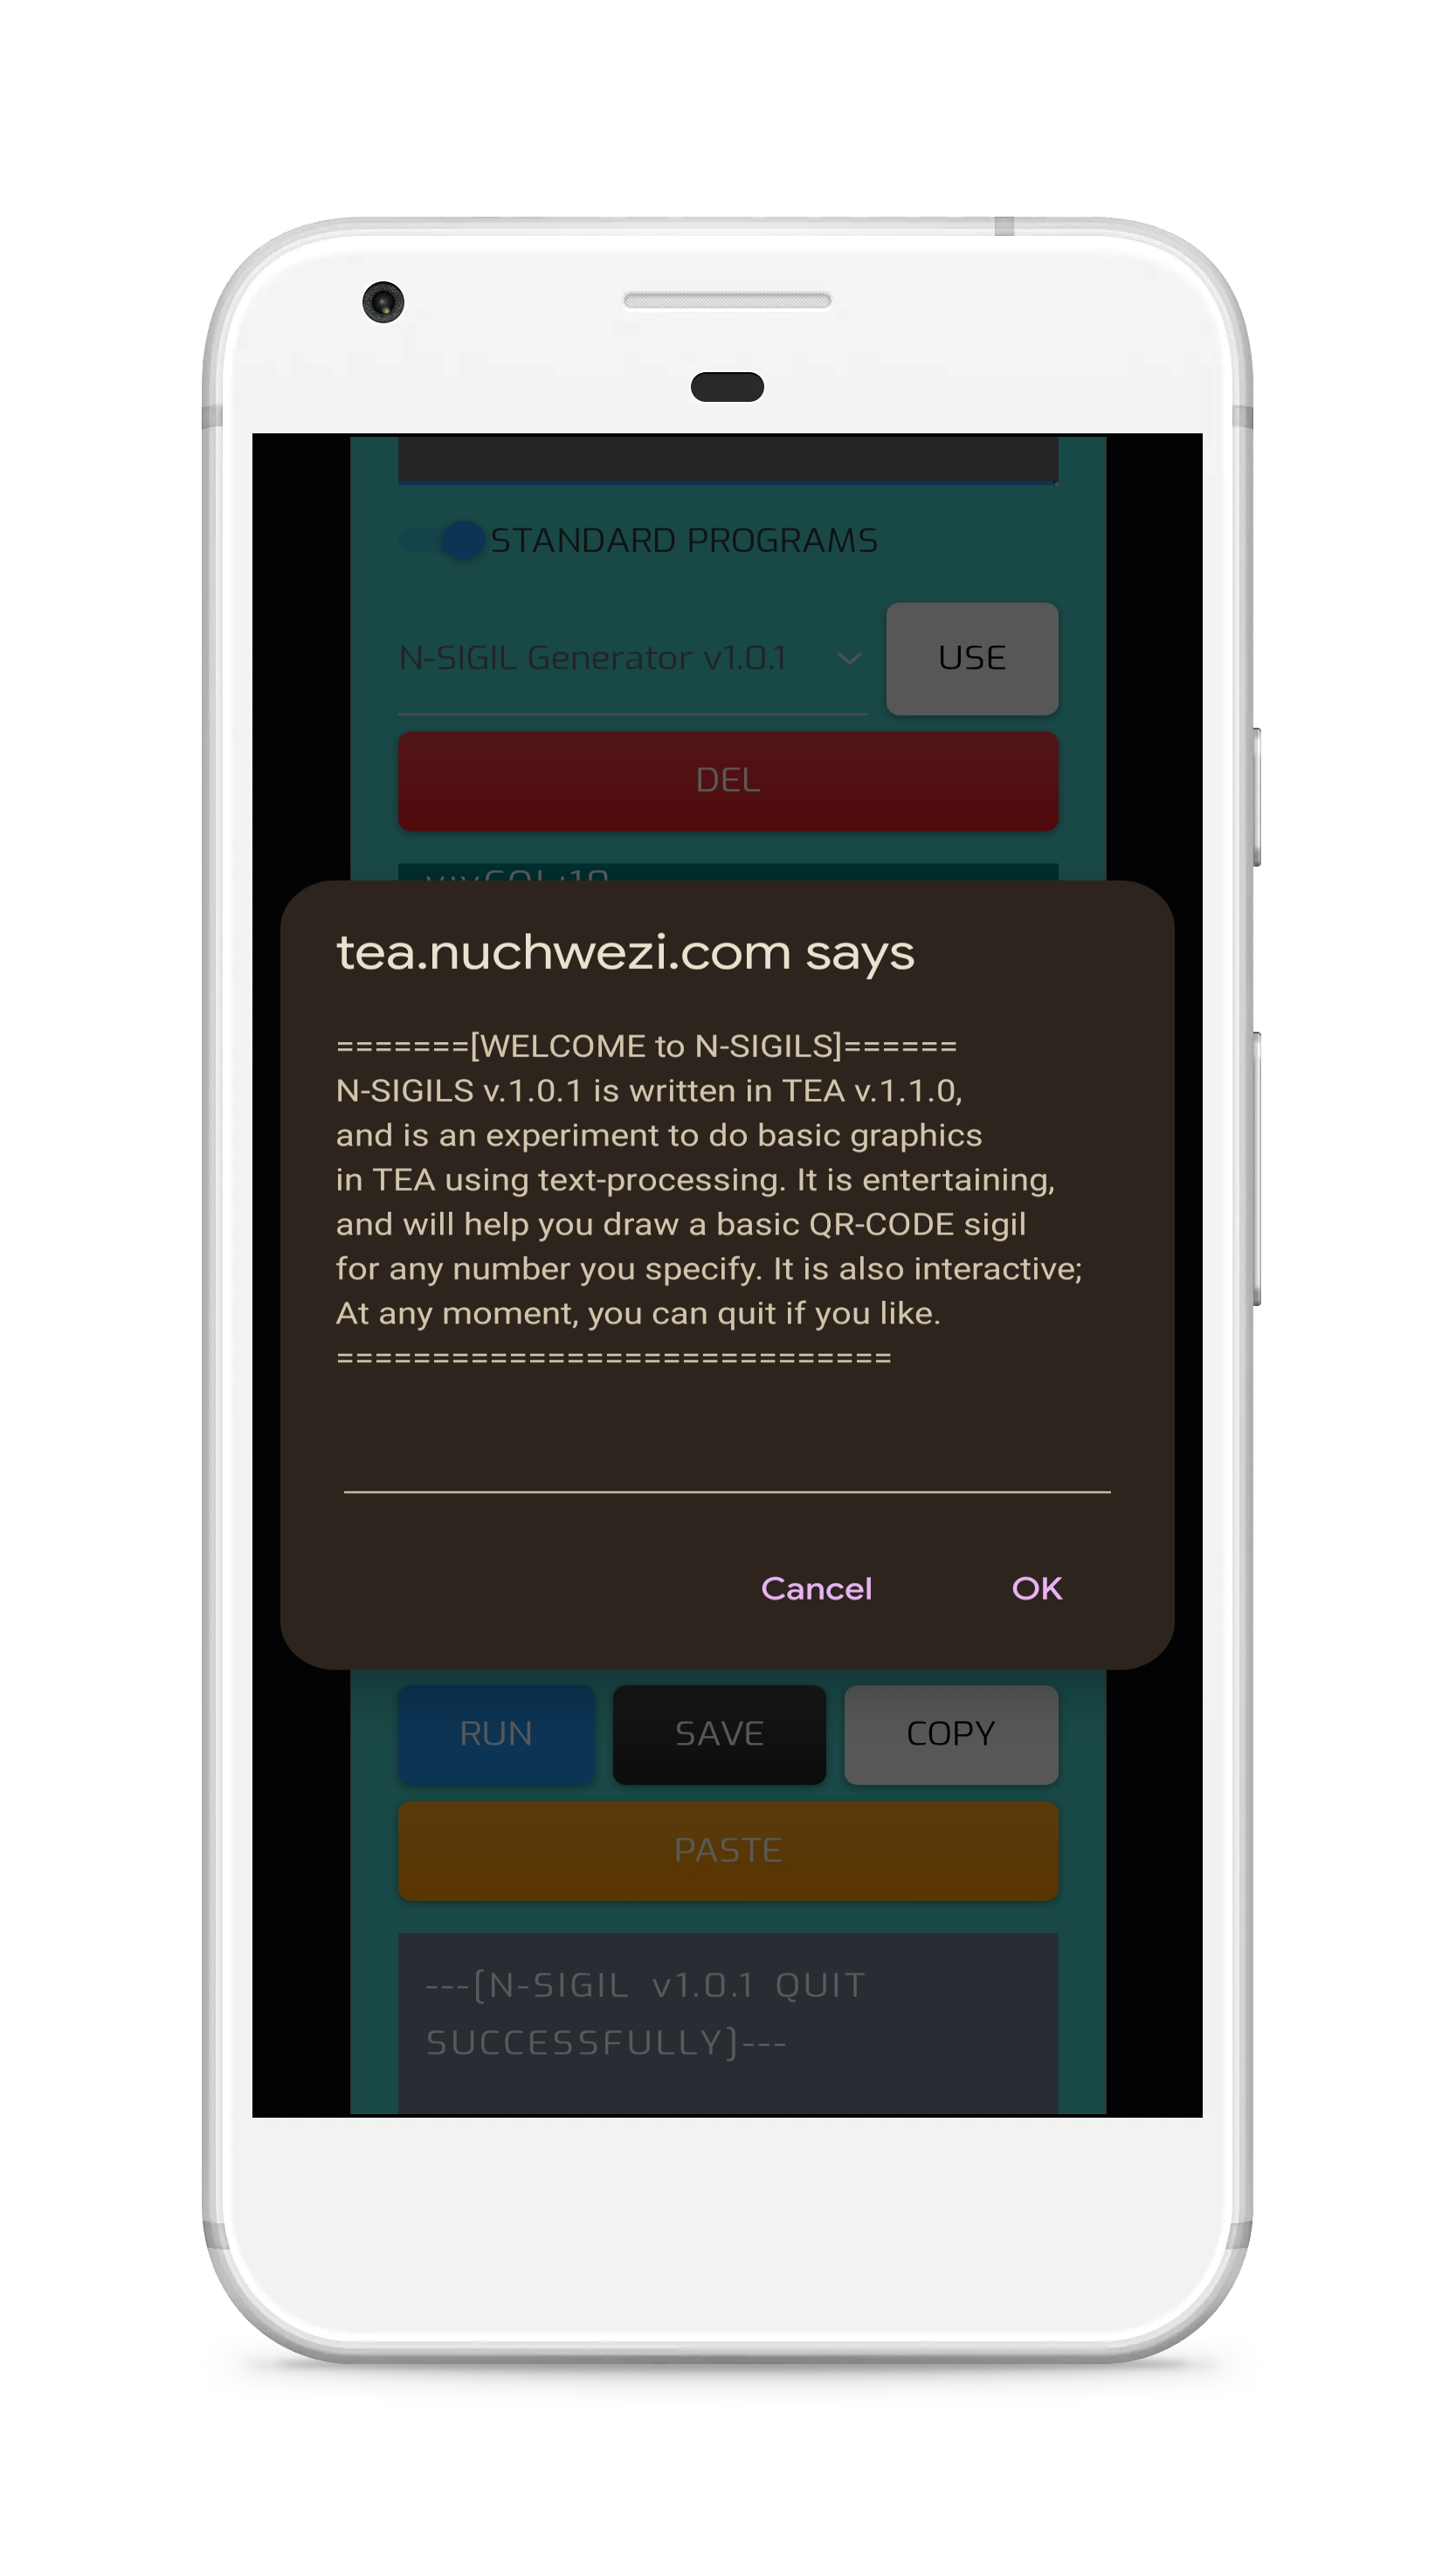
\includegraphics[width=\textwidth]{resources/images/nsigil_intro.png}
    \caption{N-SIGIL v1.0.1: Intro Greeting Interface}
    \label{FIGNSIGIL}
  \end{subfigure}
  \hfill
  \begin{subfigure}[b]{0.45\textwidth}
    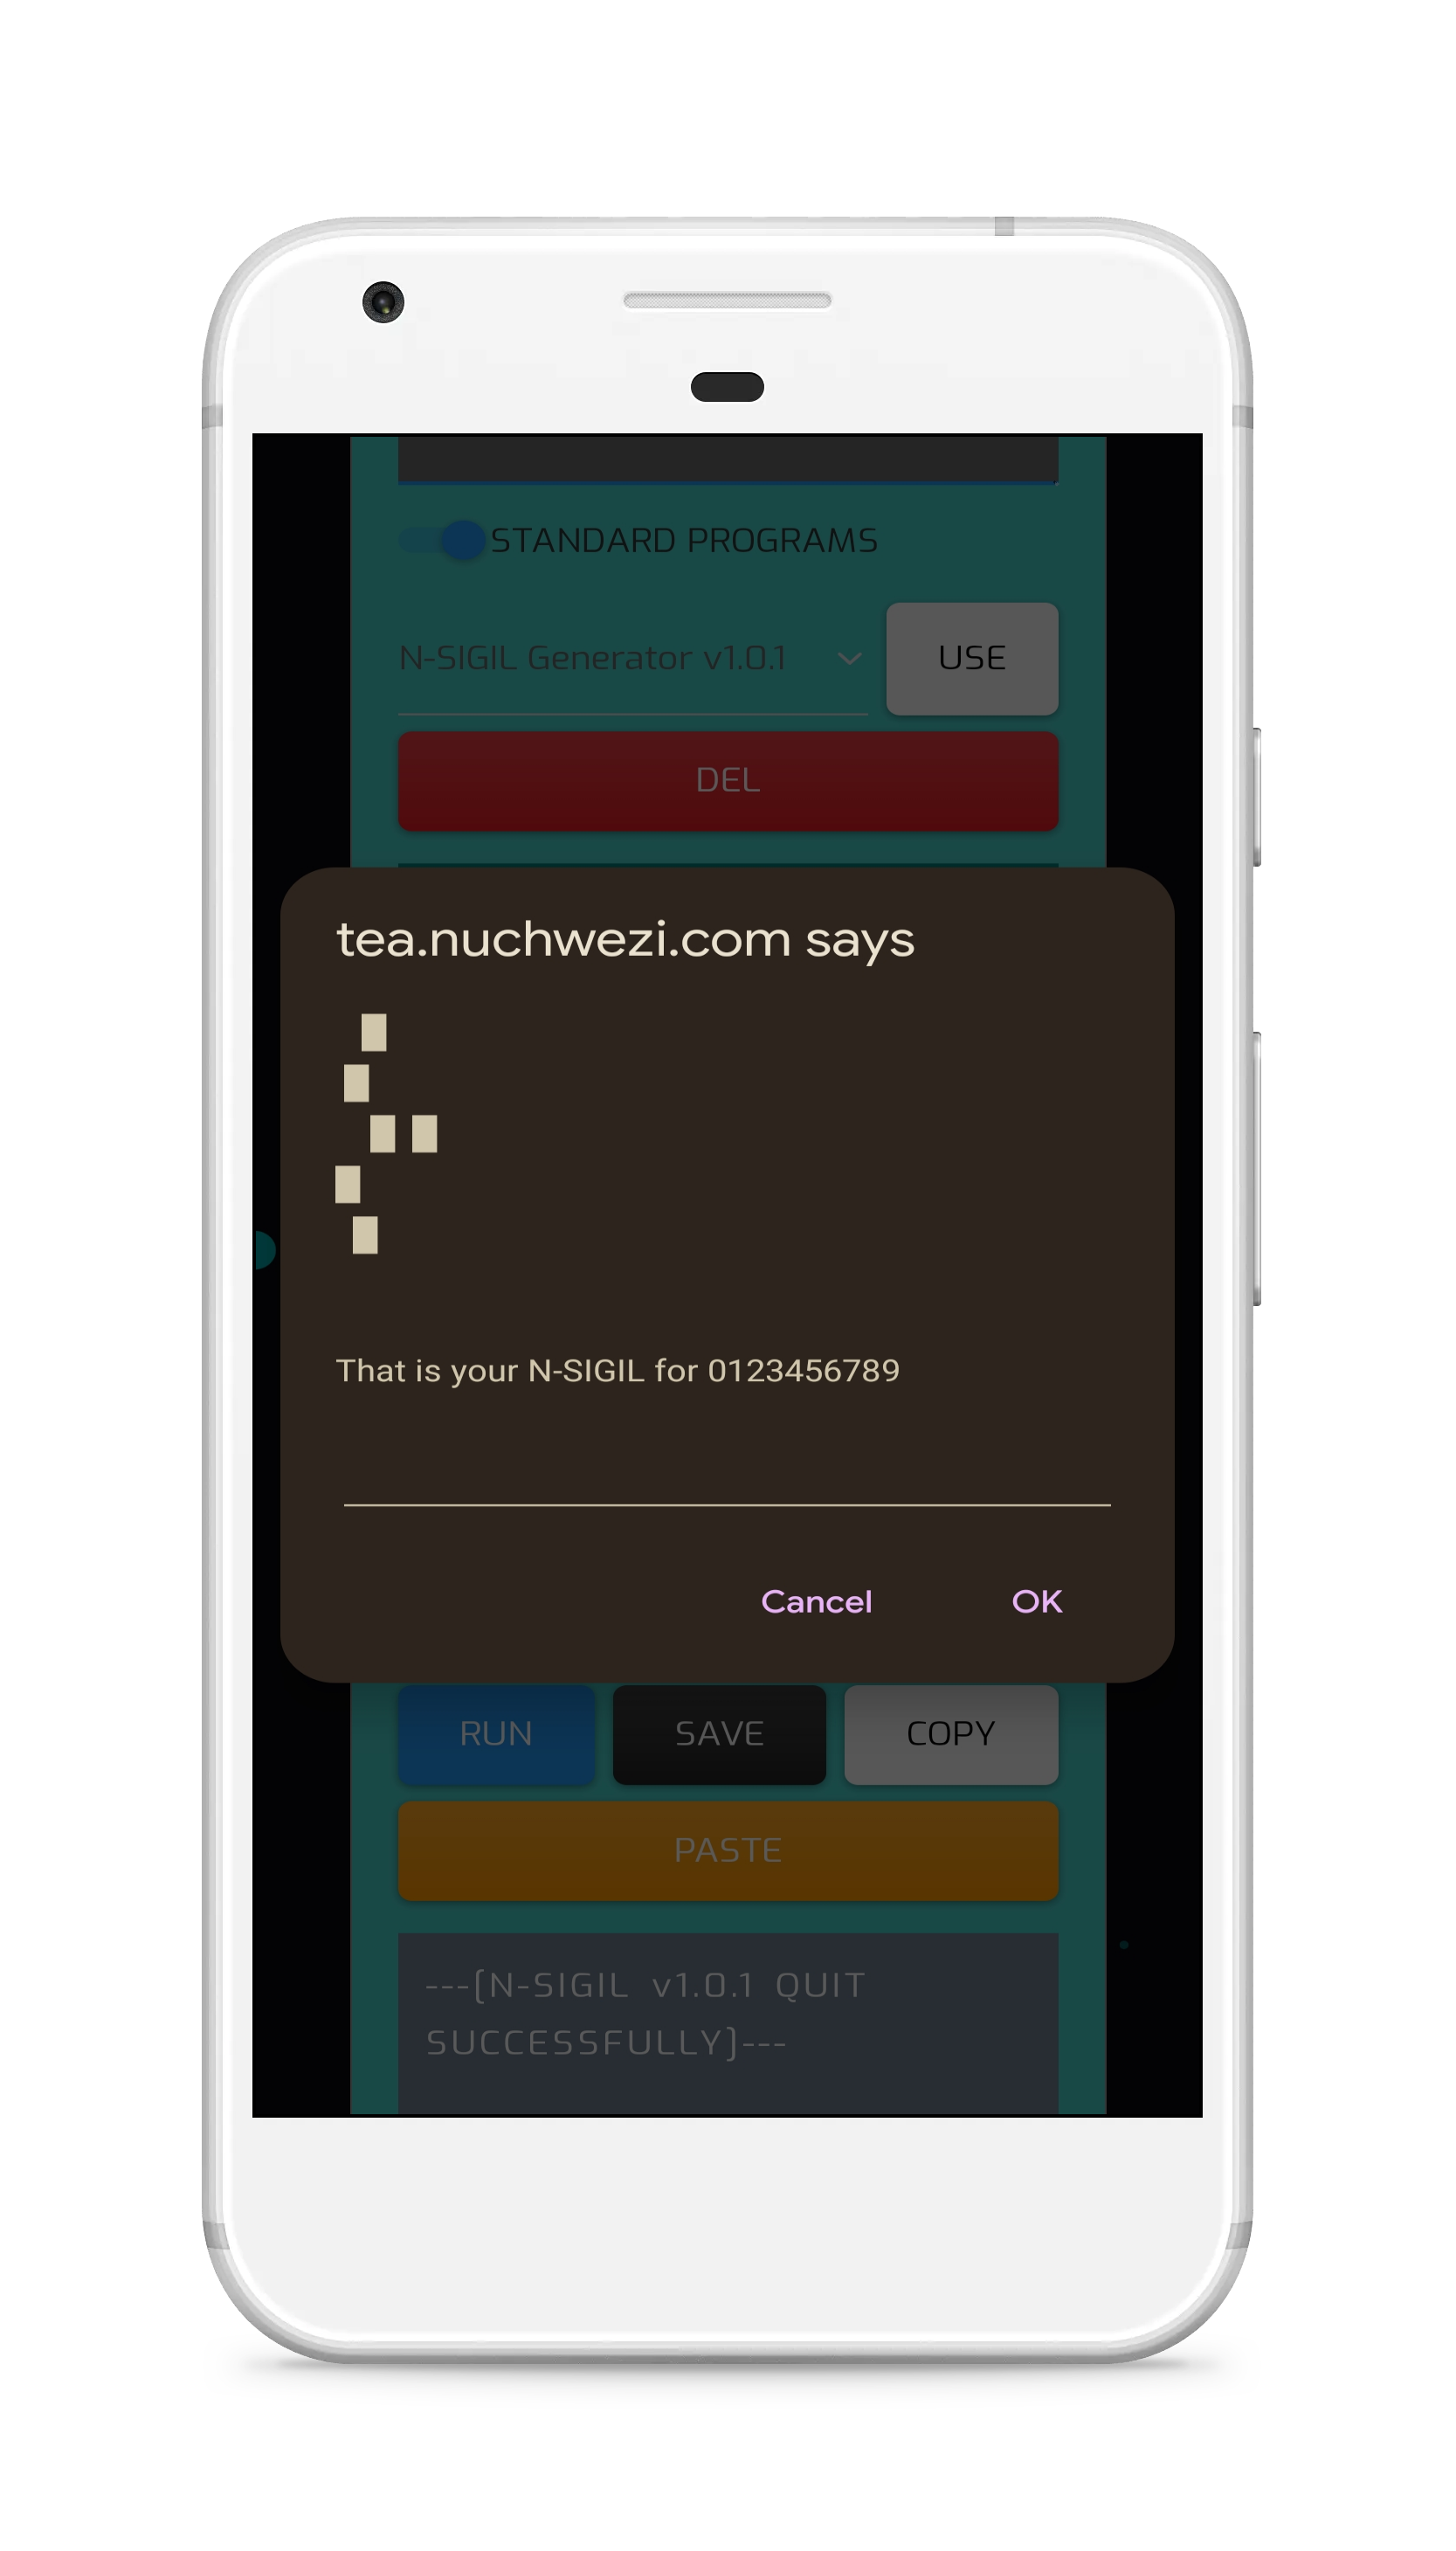
\includegraphics[width=\textwidth]{resources/images/nsigil_ossi.png}
    \caption{N-SIGIL v1.0.1: a basic qrcode for the base-10 o-SSI}
    \label{FIGNSIGIL2}
  \end{subfigure}
  \caption{Phone Snapshots of WEB TEA in action}
  \label{FIGNSIGILDEMO}
\end{figure}


    \begin{figure}[H]
      \centering
      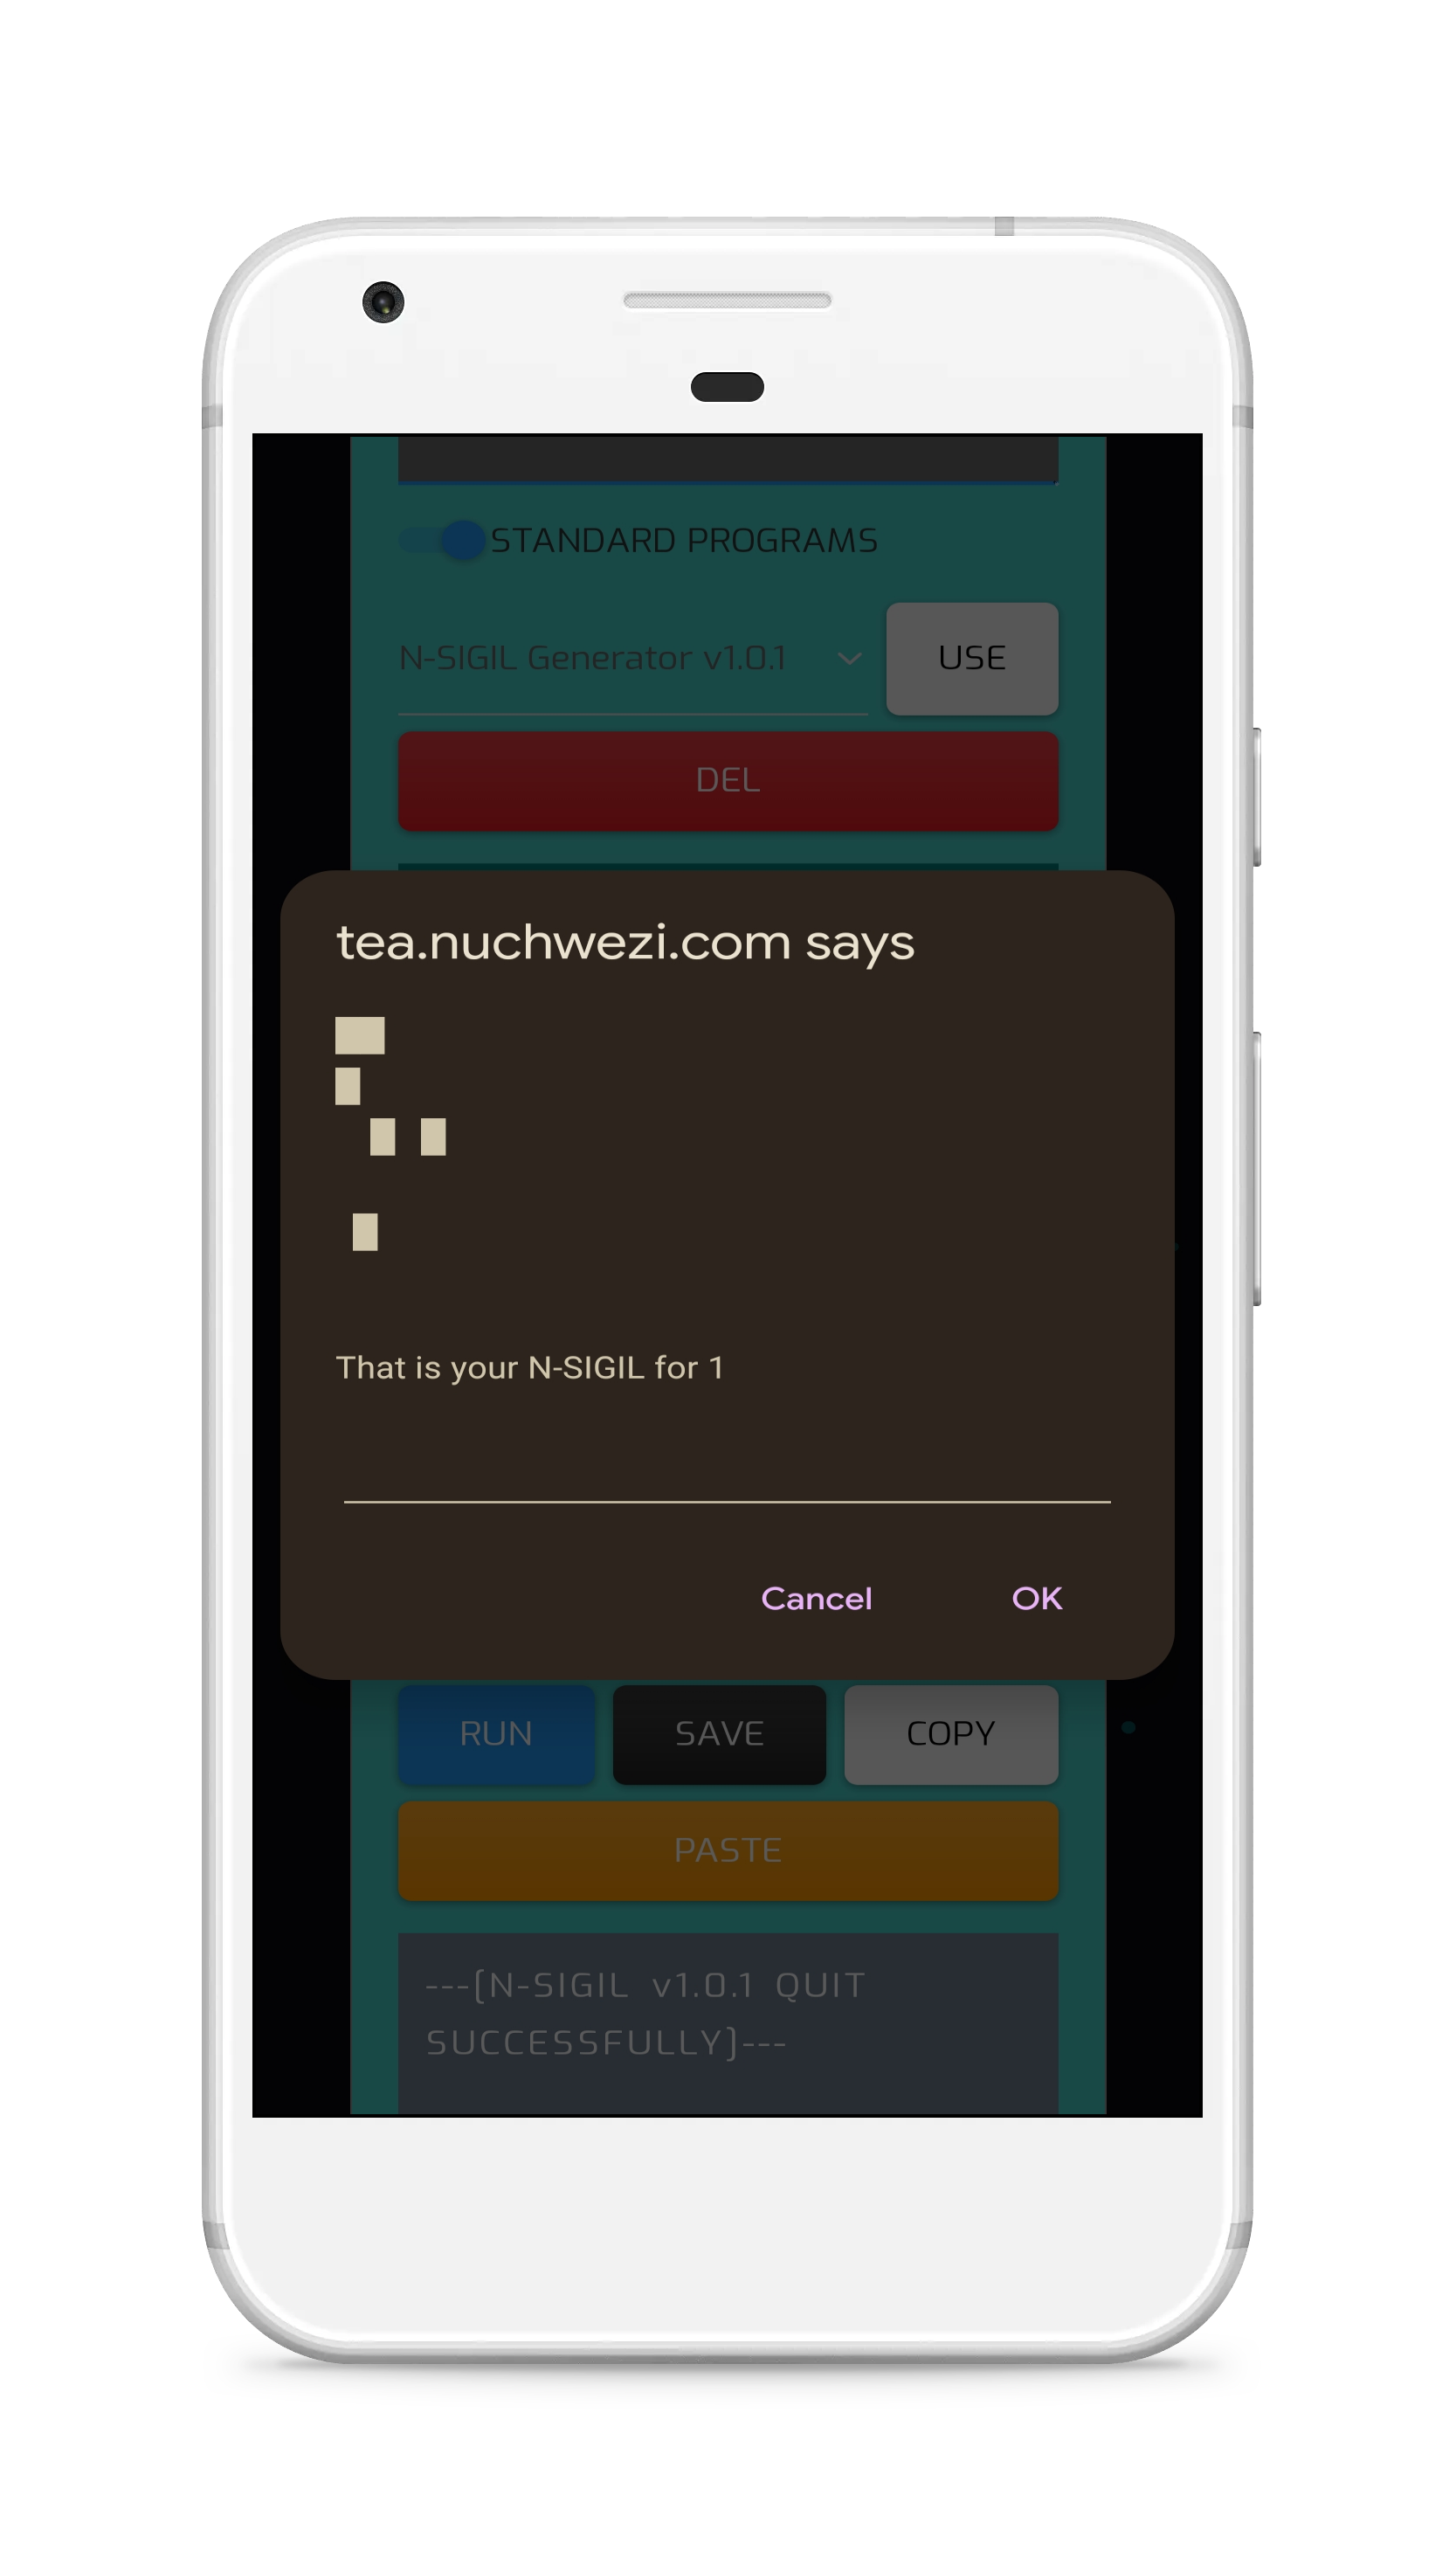
\includegraphics[height=0.6\textheight,]{resources/images/nsigil_qrcode.png}\\
        \caption{N-SIGIL v1.0.1: a basic qrcode for just the number 1}
      \label{FIGNSIGIL3}
    \end{figure}


\chapter{Conclusion}
\label{SECCONC}

%---refs fixed up to this point...


We have covered sufficient material to help anyone coming to \textbf{TEA}, to be able to understand where the language came from, what it is based on, how it is designed or specified, what the language grammar is, how the language is processed, what sample programs in the language look like, and finally, what the core aspect of the language's Instruction Set are, A: to Z:, as well as sufficient test cases and sample codes for almost each specified aspect of those 26 core TEA primitives. This book is additionally meant to serve as a manual and reference for those using TEA programming in practice, across domains, as well as those reading and trying to understand, debug or extend TEA programs. We have also include material on where, how and which TEA standard to install where, how to run or update it, as well as where to find the developers for feedback, how to join the TEA user community and also learn from and follow the inventor of the language himself.



%---[ END BOOK CONTENT/CHAPTERS ]

%---[ BEGIN BOOK END/APPENDICES]
\begin{appendices}

%\chapter{Other Functions of DNA Beyond Protein Synthesis}
%\label{APPOTHERFUNC}


%-------[ END CONTENT ]


\end{appendices}

%\includepdf[pages=1]{resources/pdfs/note_cover.pdf}

\bibliographystyle{unsrt}
\bibliography{references}

%\comment{

%\newpage

\vspace{5cm}
\fbox{
\begin{minipage}{0.9\textwidth}
\textbf{TO CITE:}\\

Lutalo, Joseph Willrich (2024). \textbf{TEA TAZ: Transforming Executable Alphabet A: to Z: COMMAND SPACE SPECIFICATION.} Figshare. Book. \url{https://doi.org/10.6084/m9.figshare.26661328}

\end{minipage}}
\\
%}


%---[ END BOOK END/BACKCOVER]

% Float the section to center of page
\begin{center}
\vspace*{\fill}

\chapter*{About the Inventor of TEA\footnote{Refer to \textbf{ORCID:} \url{https://orcid.org/0000-0002-0002-4657}}}
\addcontentsline{toc}{chapter}{About the Inventor of TEA}


\begin{figure}[H]
  \begin{center}
  %\includegraphics[trim=0cm 20cm 0cm 0cm, clip, width=0.9\textwidth,]{resources/pdfs/OZINCIPHER-APP3-EXA.pdf}\\
  %
\includegraphics[trim=LEFT BOTTOM RIGHT TOP, 
   \includegraphics[trim=0cm 1cm 0cm 2cm, clip, height=0.8\textheight,]{resources/pdfs/AboutAuthor.pdf}\\
   %\caption{The \textbf{alternative rendering}  of the same sequence as $\Omega_{veuler}$.}
  %\label{FIGLGESEULERVIRUSv2_ORIG}
  \end{center}
\end{figure}

\vspace*{\fill}
\end{center}


% insert [back] cover --- could just be a PNG or PDF
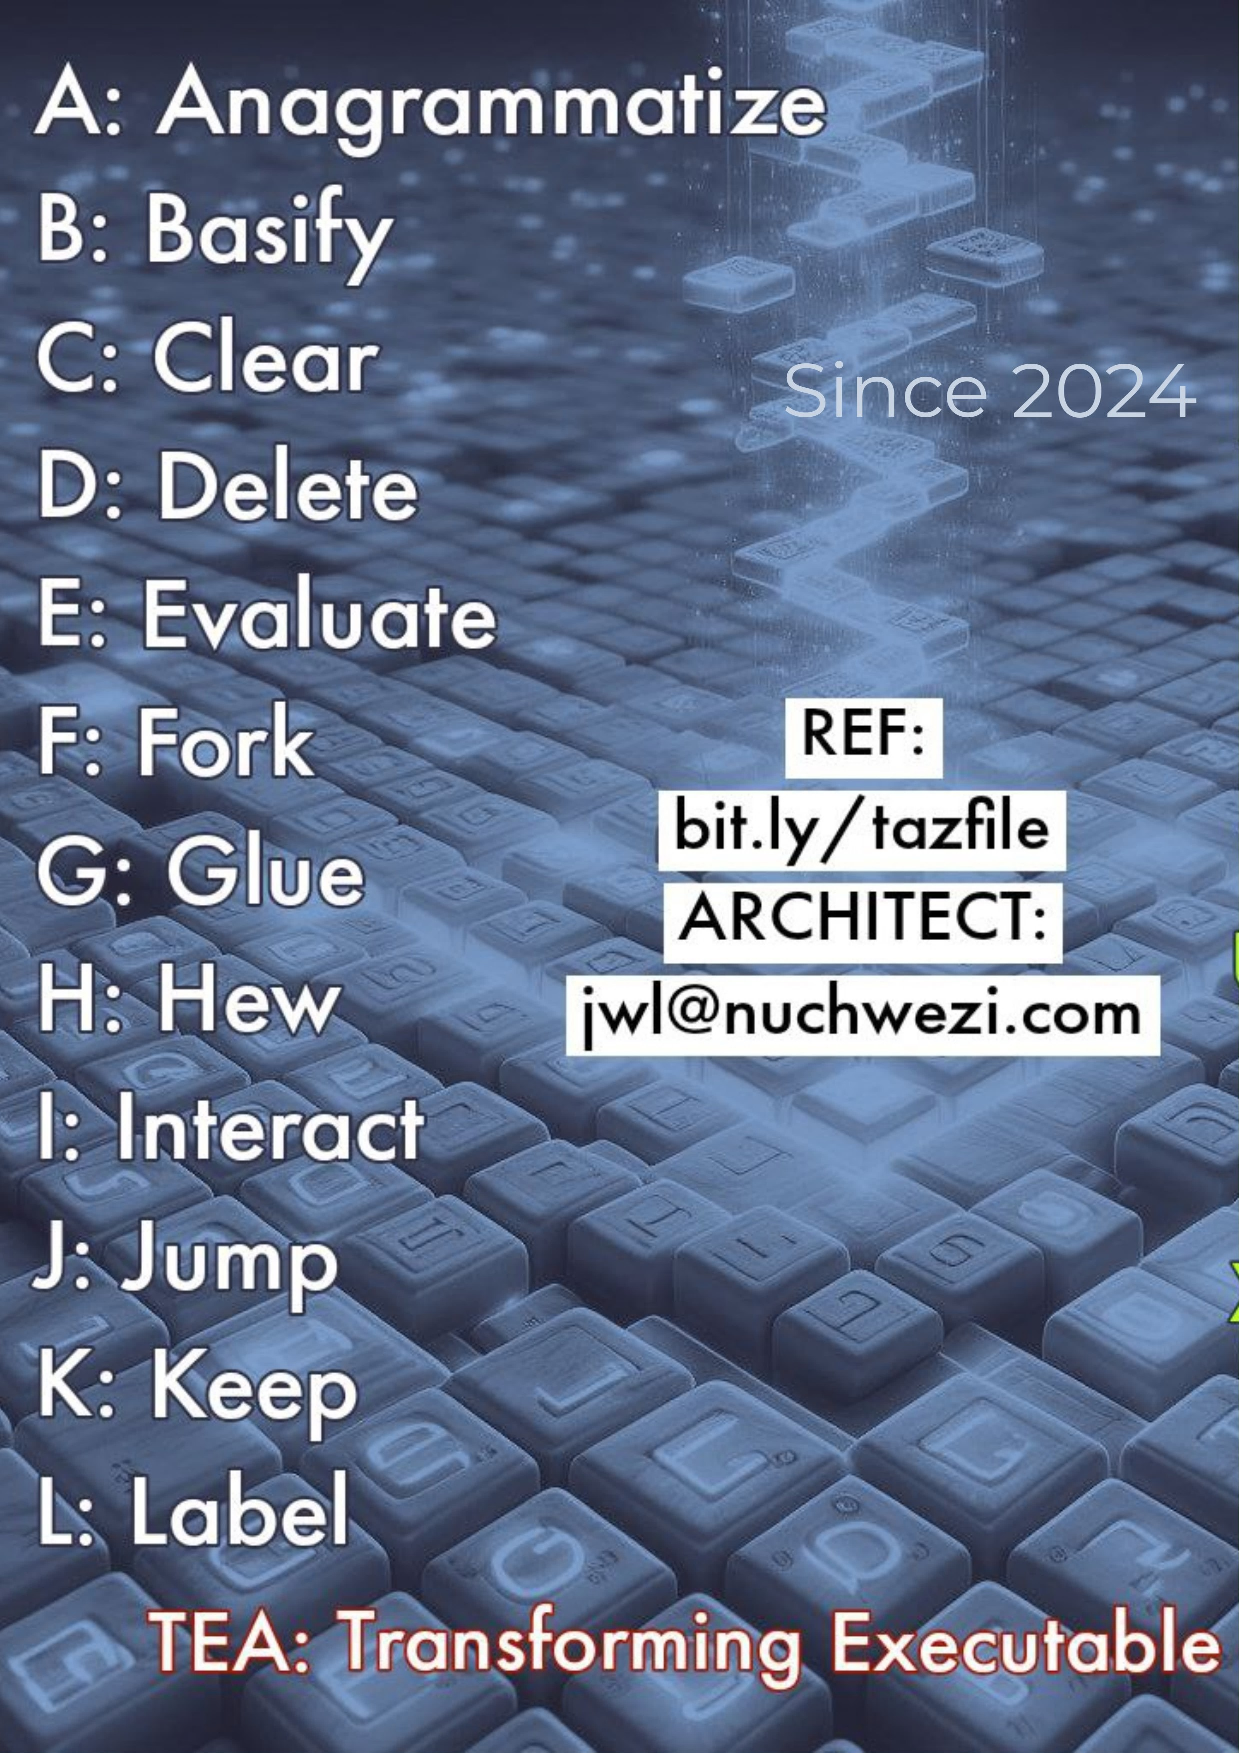
\includepdf[pages=1]{../taz_back_cover.pdf}

\end{document}